%%=============================================================================
%% Proof-Of-Concept
%%=============================================================================


\chapter{Proof-Of-Concept}%
\label{ch:Proof-Of-Concept}


In dit hoofdstuk wordt omschreven op welke manier we onderzochte technologieën hebben toegepast op de probleemstelling van het bedrijf Lockit Rentals. De werking van eigen ontwikkelde toepassingen worden specifiek toegelicht op basis van gedocumenteerde informatie. Op vlak van de QR-codes is het doel om de huidige scan software te optimaliseren. Hierbij gaan er experimenten uitgevoerd worden om deze grondig te vergelijken. In het tweede deel zal de chatbot ontwikkeld worden aan de hand van het gekozen platvorm. Om aan te tonen dat nieuwe technieken een oplossing kunnen bieden, verwijs ik door naar de verwerkte resultaten \ref{ch:verwerkingresultaten}.

\section{Opbouw experimenten}%
\label{sec:toepassingenQR-coce scanners}

Zowel de nieuwe als de oude opstelling worden grondig getest in vier verschillende scenario’s. Daarnaast zijn er ook twee manieren om de toegangscode te bezitten. Allereerst kan de klant in het bezit zijn van een QR-code op papier. Alsook kunnen ze deze digitaal op de Lockit Rentals mobiele applicatie registreren. Beide manieren laat scan mogelijkheden toe. Dit zal een rol spelen in de aantal uitgevoerde experimenten waarbij constante variabelen van toepassing zijn. De QR-code dat gescand wordt door dezelfde testpersoon op hetzelfde apparaat zorgen voor betrouwbaar eindresultaat. 
Aangezien sommige omgevingsfactoren veranderen doorheen het proces zullen we ook de verlichtingssterkte meten uitgedrukt in lux. Deze waarde zal niet meegenomen worden bij de conclusie maar is gewoon ter illustratie. 
Op het einde van elke test wordt er een \ac{XLSX} bestand gecreëerd. Een voorbeeld hiervan is te zien op figuur \ref{fig:xlsxBestandExperiment}. Deze bestanden hebben steeds een logische naamgeving zodat we dit later kunnen verwerken in een duidelijke conclusie. In figuur x zien we de oplijsting van alle bestanden.


\begin{figure}
    \centering
    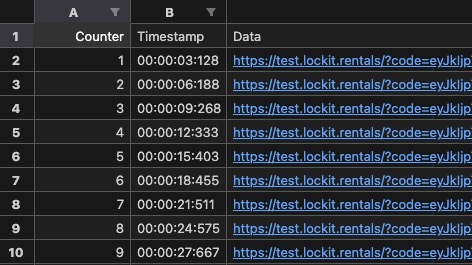
\includegraphics[width=0.8\textwidth]{graphics/F27_QR-data_uitlezing.jpg}
    \captionsetup{justification=centering, singlelinecheck=false}    
    \caption{Voorbeeld \ac{XLSX} bestand na uitvoeren van QR-code camera programma.}
    \label{fig:xlsxBestandExperiment}
\end{figure}}

\begin{figure}
    \centering
    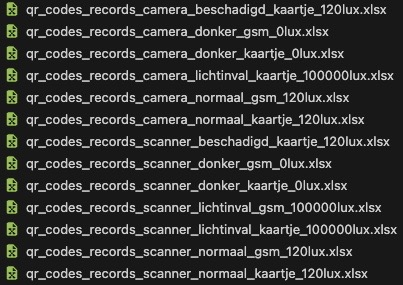
\includegraphics[width=0.8\textwidth]{graphics/F28_XLSX_opsomming.jpg}
    \captionsetup{justification=centering, singlelinecheck=false}    
    \caption{Opsomming alle \ac{XLSX} bestanden na uitvoeren van QR-code camera programma.}
    \label{fig:opsomming}
\end{figure}}


\section{Experiment 1: Huidige QR-camera}
\label{sec:huidigeToepassingScanners}

In het hoofdstuk \ref{sec:WerkingUnits} wordt aangetoond welk script er effectief actief is op de locker units. Na grondig onderzoek van de gebruikte camera’s kunnen we concluderen dat deze geen specifieke toestellen zijn om QR-codes te scannen. De camera op zich heeft veel configuratie en rekenkracht nodig om de QR-code waar te nemen en te kunnen capteren in bruikbare data. 

Om deze experimenten uit te voeren, ga ik gebruik maken van een eigen opstelling die de huidige scanner inclusief de software hanteert te zien op figuur \ref{fig:vooraanzichtUSBCamera} en \ref{fig:achteraanzichtUSBCamera}. Uiteraard maak ik enkele aanpassingen aan de code om ervoor te zorgen dat deze geschikt is voor de vergelijking.  Het is belangrijk om op te merken dat deze wijzigingen geen invloed zullen hebben op de eindresultaten van de experimenten. Deze aangepaste code wordt weergegeven in listing \ref{lst:huidigeQR-codeData}.

\begin{figure}[h]
    \centering
    \begin{minipage}{0.45\textwidth}
        \centering
        \rotatebox{-90}{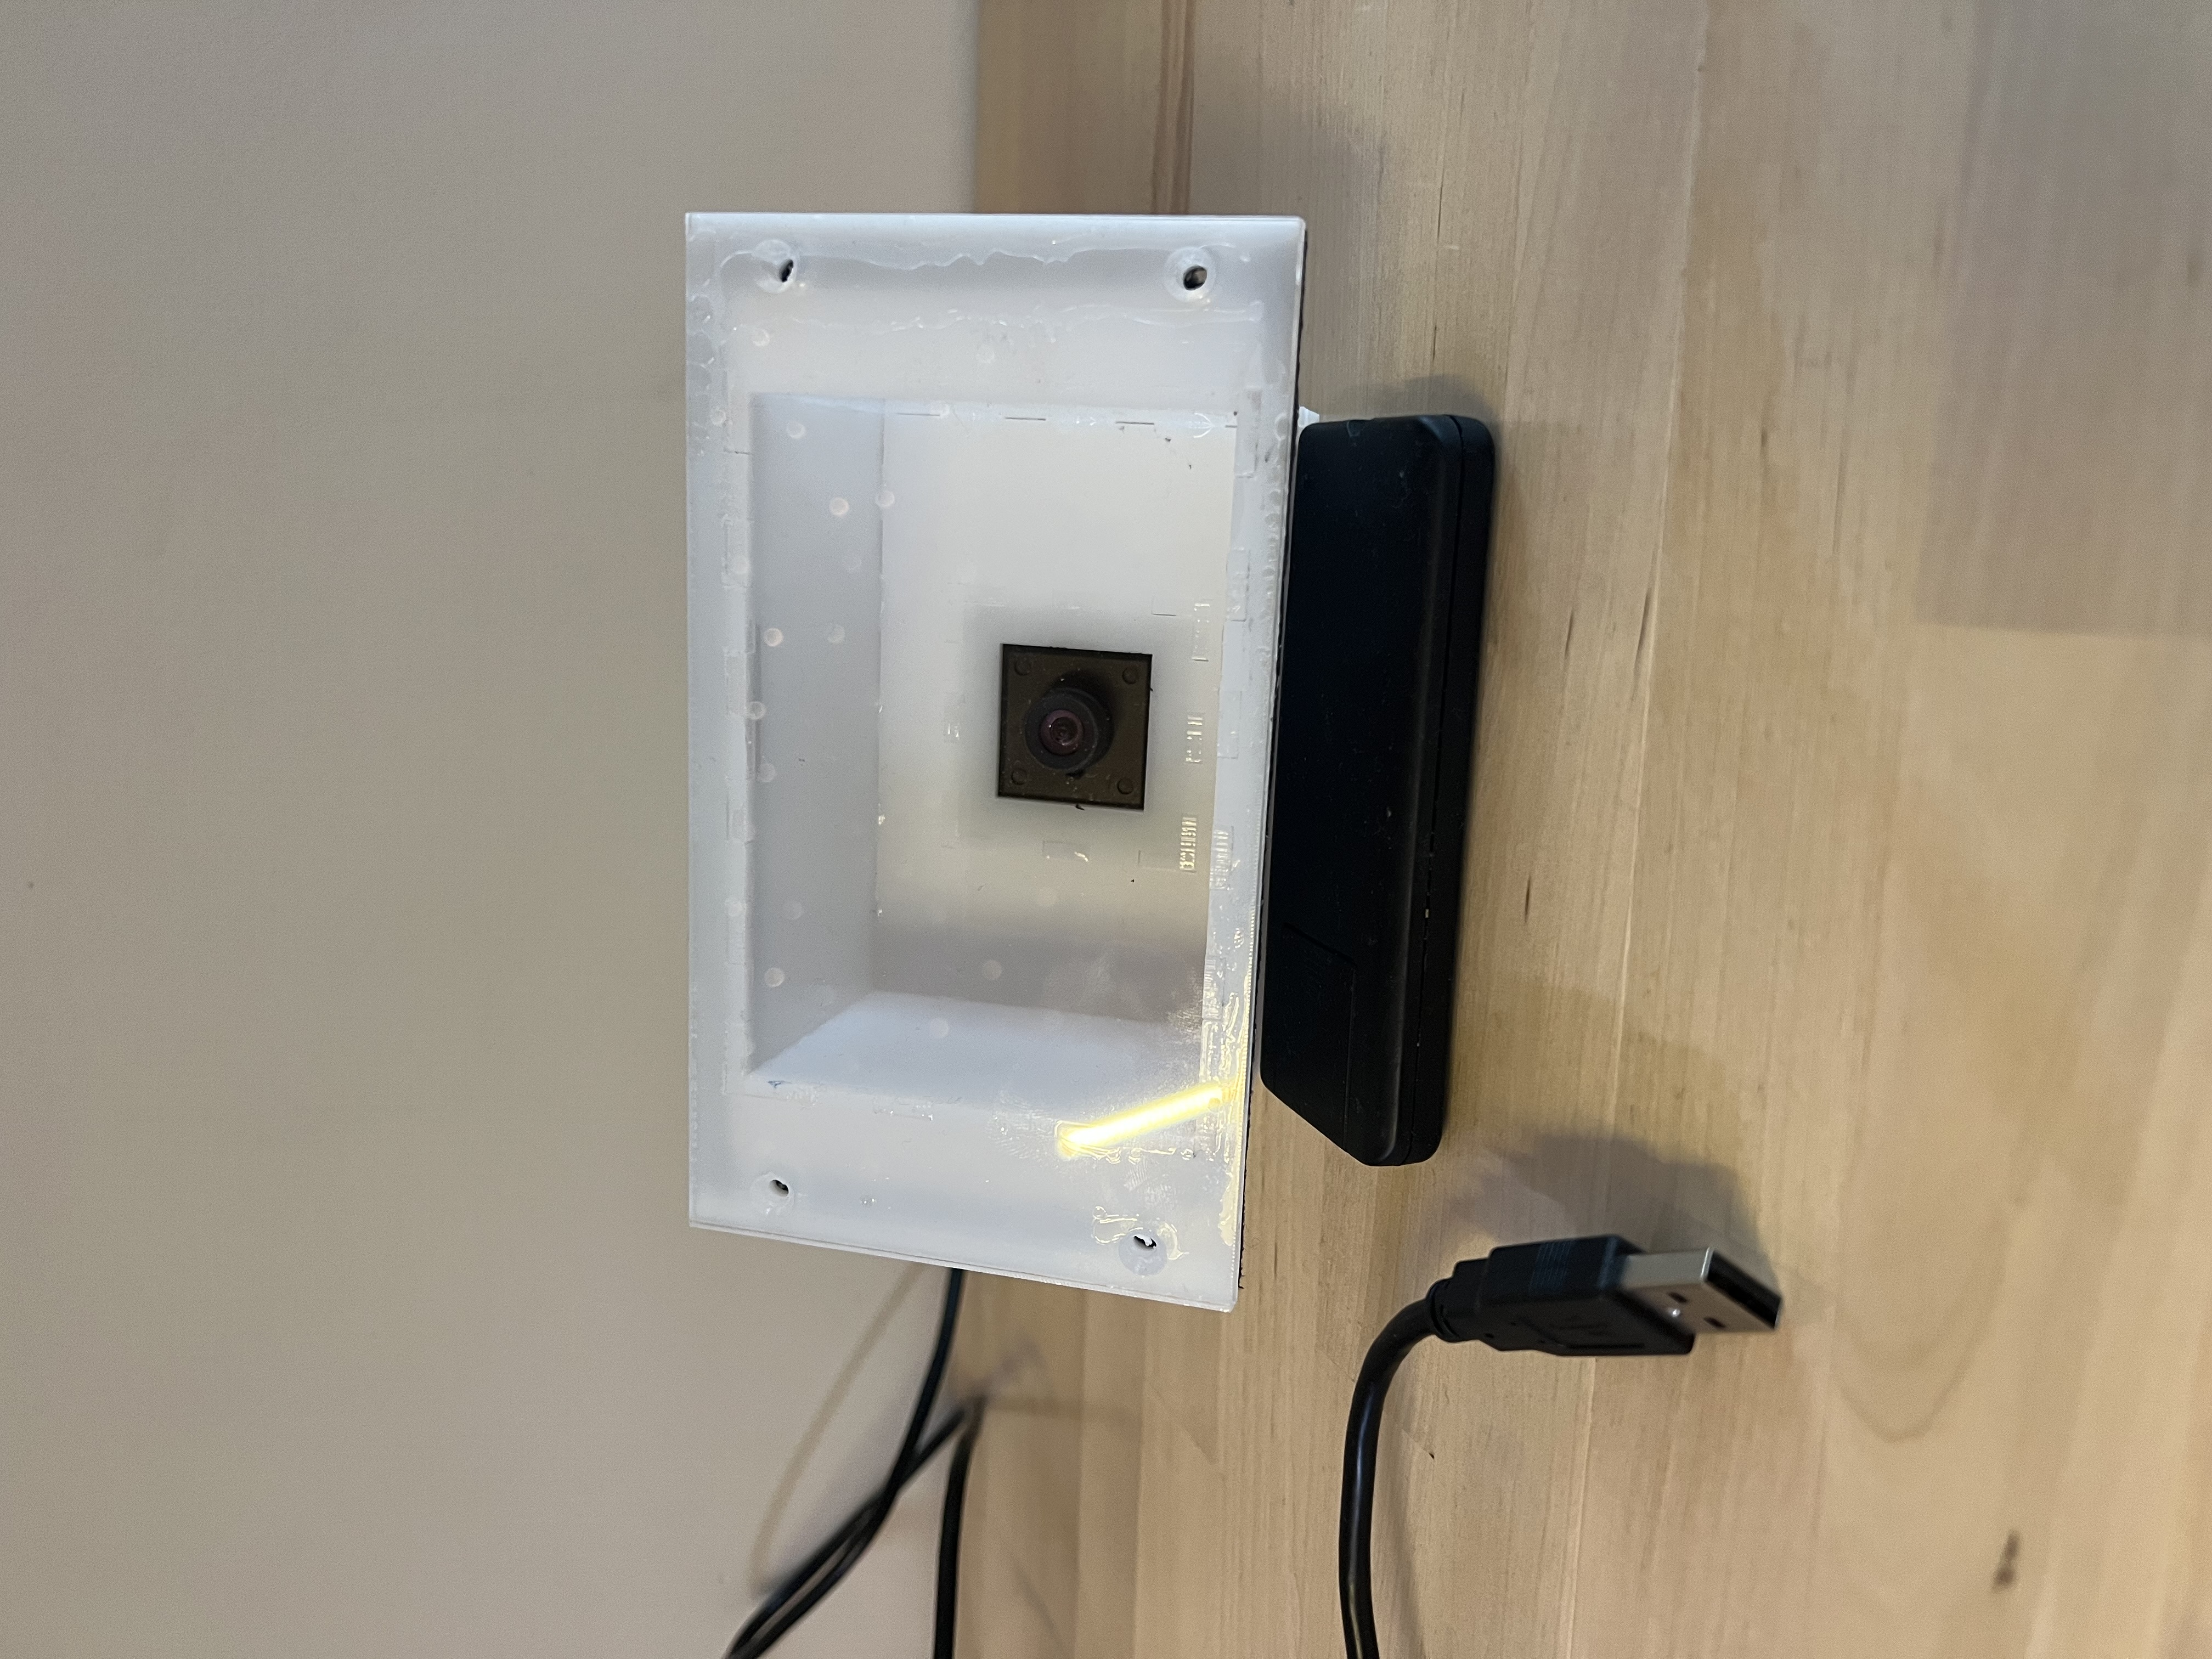
\includegraphics[width=\textwidth]{graphics/F22_USBCamera_front.jpeg}}
        \caption{Vooraanzicht USB QR-camera}
        \label{fig:vooraanzichtUSBCamera}
    \end{minipage}
    \hfill
    \begin{minipage}{0.45\textwidth}
        \centering
        \rotatebox{-90}{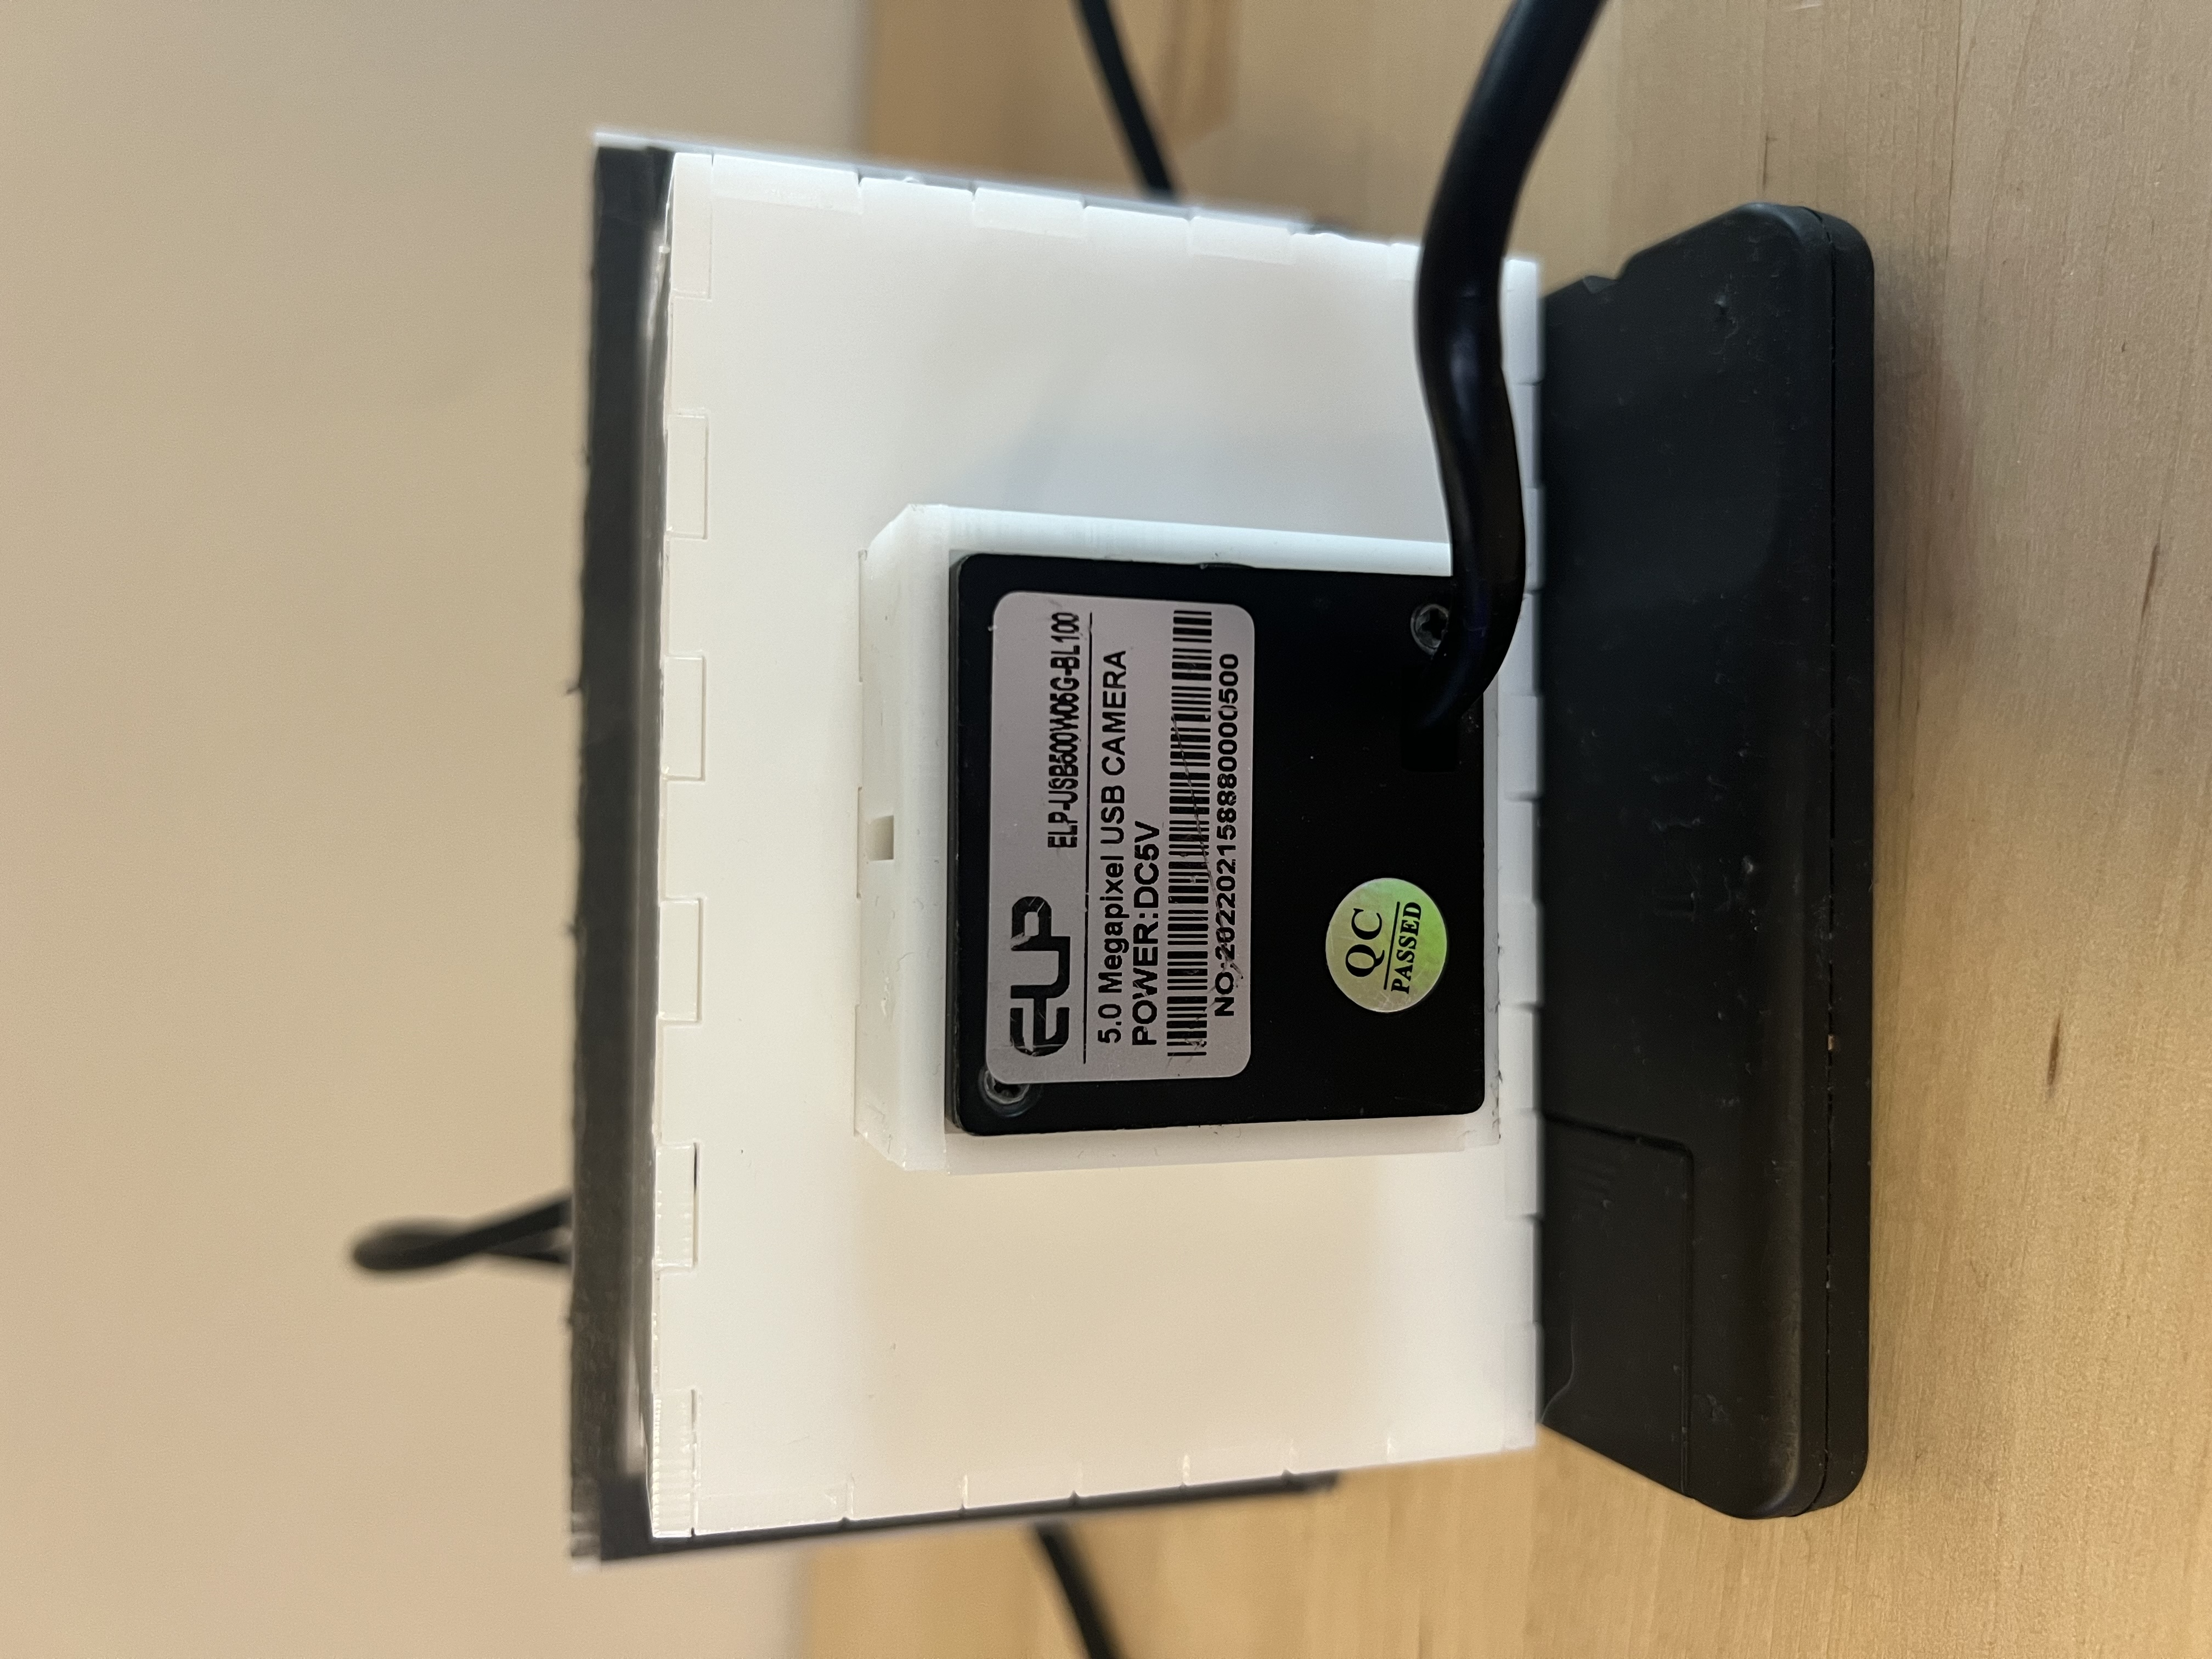
\includegraphics[width=\textwidth]{graphics/F23_USBCamera_back.jpeg}}
        \caption{Achteraanzicht USB QR-camera}
        \label{fig:achteraanzichtUSBCamera}
    \end{minipage}
\end{figure}


\begin{lstlisting}[language=Python, caption={Python script voor experiment van QR-code camera.}, label=lst:huidigeQR-codeData, numbers=left]
    import cv2  # Importeer de cv2-bibliotheek voor het werken met beeldverwerking
    import time  # Importeer de time-bibliotheek om pauzes in de uitvoering van het programma te creëren
    import pyzbar.pyzbar as pyzbar  # Importeer de pyzbar-bibliotheek voor het decoderen van QR-codes
    from datetime import datetime  # Importeer de datetime-bibliotheek om tijdstempels te maken
    from openpyxl import Workbook  # Importeer de openpyxl-bibliotheek voor het werken met Excel-bestanden
    
    camera = cv2.VideoCapture(0)  # Gebruik de cv2-bibliotheek om toegang te krijgen tot de camera
    counter = 1  # Initialiseer een teller om bij te houden hoeveel QR-codes zijn gescand
    start_time = datetime.now()
    
    # Maak een nieuw werkboek / excel aan en selecteer het actieve werkblad
    workbook = Workbook()
    worksheet = workbook.active
    # Stel de kolomkoppen in voor het Excel-bestand
    worksheet['A1'] = 'Counter'
    worksheet['B1'] = 'Timestamp'
    worksheet['C1'] = 'Data'
    
    def decode_qr(image):  # Functie om QR-codes te decoderen
        try:
            gray = cv2.cvtColor(image, cv2.COLOR_BGR2GRAY)  # Zet het kleurenbeeld om in grijswaarden
            barcodes = pyzbar.decode(gray, symbols=[pyzbar.ZBarSymbol.QRCODE])  # Decodeer QR-codes
            if barcodes:
                timestamp = (datetime.now() - start_time).total_seconds()  # Bereken het tijdsverschil vanaf het begin
                timestamp_formatted = time.strftime('%H:%M:%S:%f', time.gmtime(timestamp))  # Maak de tijdstempel
                return (barcodes[0].data.decode(), timestamp_formatted)  # Return de gedecodeerde gegevens en tijdstempel
        except Exception as e:
            print(e)
        return None
    
    while counter <= 50:
    ret, frame = camera.read() # Lees de afbeelding van de camera
    
        if not ret:
            break
        qr_data = decode_qr(frame) # Decodeer QR-code in afbeelding
        if qr_data:
            timestamp = (datetime.now() - start_time).total_seconds() * 1000 # Formatteer de timestamp
            hours, remainder = divmod(int(timestamp), 3600000)
            minutes, remainder = divmod(remainder, 60000)
            seconds, milliseconds = divmod(remainder, 1000)
            timestamp_formatted = f"{hours:02}:{minutes:02}:{seconds:02}:{milliseconds:03}"
            # Print de QR-code informatie en voeg het toe aan de Excel-sheet
            print(f'{counter} | Timestamp: {timestamp_formatted} | Data: {qr_data[0]}')
            # Normaal doen we hier het POST request naar de server zie originele code
            row = (counter, timestamp_formatted, qr_data[0])
            worksheet.append(row)
            counter += 1
        time.sleep(3) # Wacht 3 seconden tussen elke frame
    
    
    end_time = datetime.now()
    
    # Sla het Excel bestand op
    workbook.save('qr_codes_records_camera_normaal_gsm_120lux.xlsx')
    
    print(f"Counter reached {counter - 1}. Exiting program. Final time of scanning: {end_time - start_time}")
    camera.release() # Beëindig het gebruik van de camera    
\end{lstlisting}

\subsection{Resultaten huidig QR-camera experiment}
\label{sec:huidigeToepassingScannersExperiment}

Hieronder bevinden zich de tabellen met daarin de eindresultaten van het experiment met de huidige QR-camera. Er zijn telkens 50 QR-codes gescand met uitzondering van QR-codes in de beschadigde situatie.

\begin{table}[h]
    \centering
    \begin{tabular}{ c|c|c|c }
        \cline{2-4}
        & \textbf{\textit{QR-code op papier}} & \textbf{\textit{QR-code op gsm}} & \textbf{\textit{Verlichtingssterkte}} \\
        \cline{2-4}        
        \hline
        \textbf{\textit{1. Normaal}} &  230,402 s & 189,09 s & 120 lux \\
        \hline
        \textbf{\textit{2. Lichtinval}} & 204,729 s & 275,128 s & 100.000 lux \\
        \hline
        \textbf{\textit{3. Donker}} & 517,394 s & 166,856 s & 5 lux \\
        \hline        
    \end{tabular}
    \captionsetup{justification=centering}
    \caption{De waarden in de tabel zijn uitgedrukt in milliseconden (ms). Geef de resultaten weer van de huidige QR-camera experiment.}
    \label{tab:3expeQR-camera}
\end{table}

Het experiment dat beschadigde QR-codes omvat zal doorgaan met een set van acht QR-codes die beschadigd of onleesbaar gemaakt zijn. Deze QR-codes zijn zichtbaar op figuur \ref{fig:beschadigdeQR-codes} en zijn gerangschikt op basis van toenemende mate van beschadiging.

\begin{table}[h]
    \centering
    \begin{tabular}{ c|c }
        \cline{2-2}
        & \textbf{\textit{Beschadigd}} \
        \cline{2-2}
        \textbf{\textit{QR-code 1}} & 3,178 s \
        \cline{2-2}
        \textbf{\textit{QR-code 2}} & 15,588 s \
        \cline{2-2}
        \textbf{\textit{QR-code 3}} & 21,788 s \
        \cline{2-2}
        \textbf{\textit{QR-code 4}} & 99,403 s \
        \cline{2-2}
        \textbf{\textit{QR-code 5}} & / \
        \cline{2-2}
        \textbf{\textit{QR-code 6}} & / \
        \cline{2-2}
        \textbf{\textit{QR-code 7}} & / \
        \cline{2-2}
        \textbf{\textit{QR-code 8}} & 158,377 s \
        \cline{2-2}
    \end{tabular}
    \captionsetup{justification=centering}
    \caption{De waarden in de tabel zijn uitgedrukt in seconden (s). De verlichtingssterkte bij deze uitwerking is 120lux. De QR-codes in kwestie zijn te vinden in figuur \ref{fig:beschadigdeQR-codes}.}
    \label{tab:omgezette_tabel_seconds}
\end{table}

\begin{figure}
    \centering
    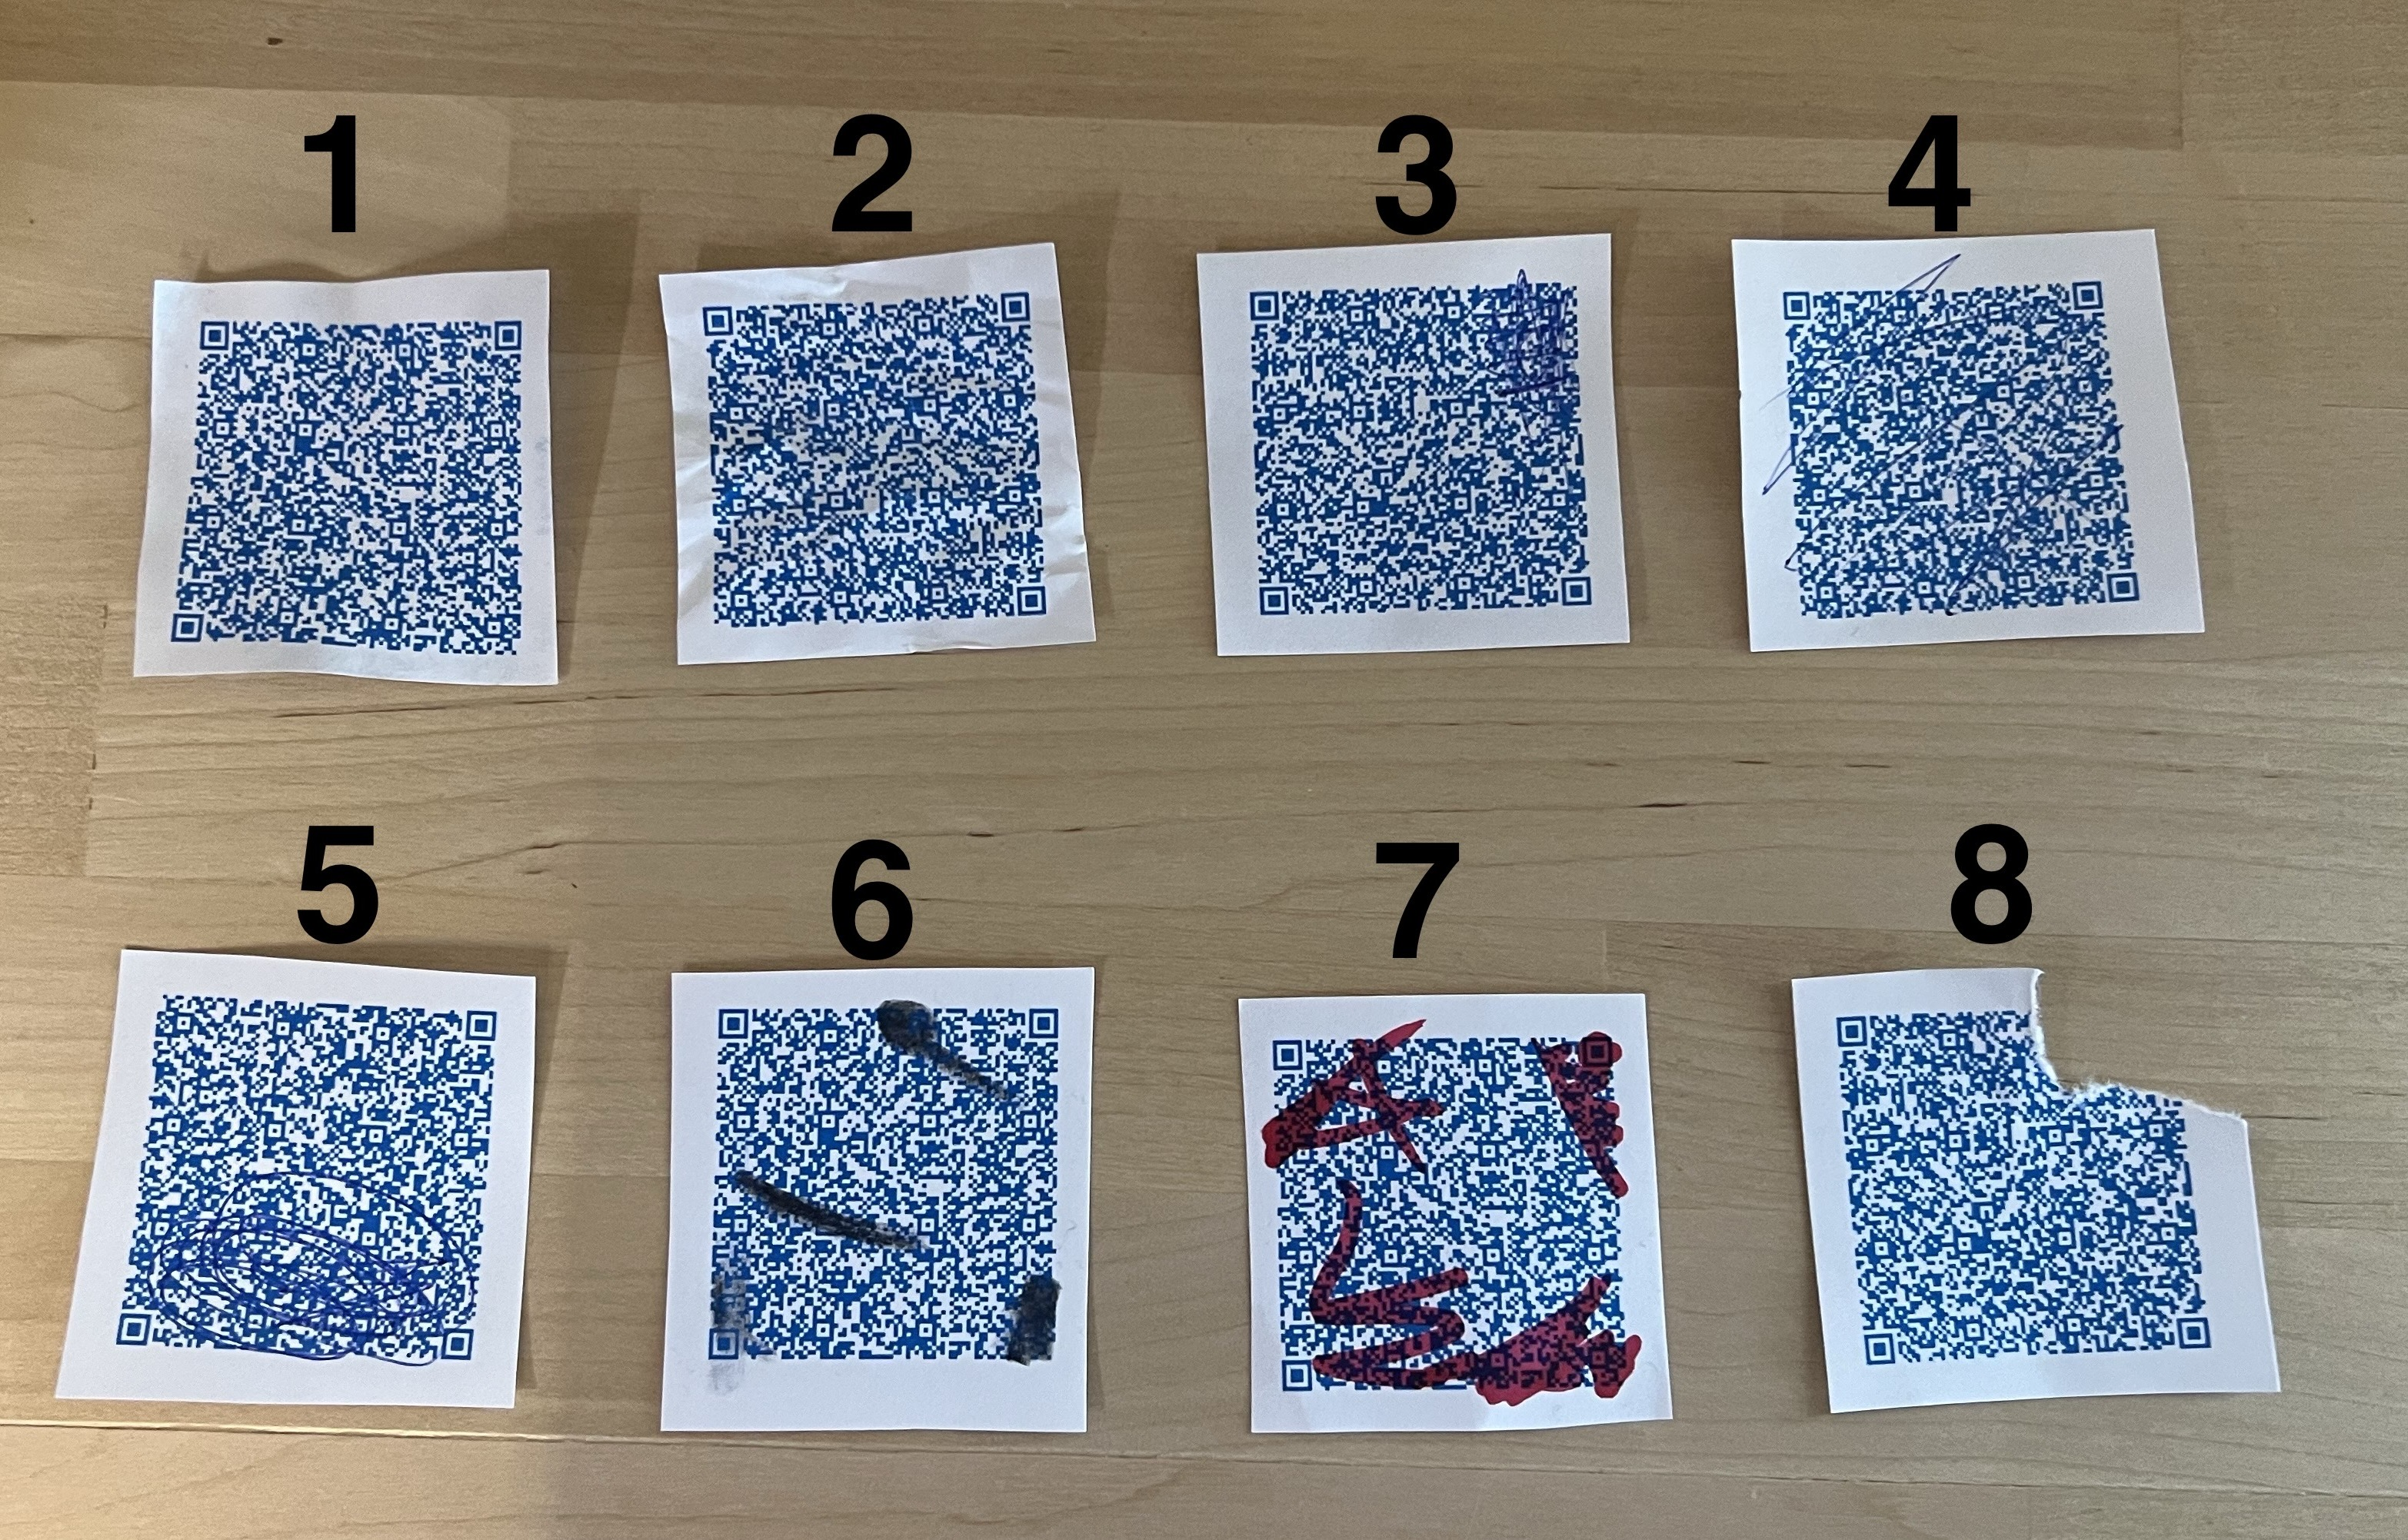
\includegraphics[width=0.8\textwidth]{graphics/F33_setBeschadigdeQR-codes.jpeg}
    \captionsetup{justification=centering, singlelinecheck=false}    
    \caption{Set van acht beschadigde QR-codes gerangschikt op basis van toenemende mate van beschadigde.}
    \label{fig:beschadigdeQR-codes}
\end{figure}}

\section{Experiment 2: Uitwerking nieuwe QR-scanner}
\label{sec:nieuweToepassing}

Wat opvalt bij het herschrijven en aanpassen van de bestaande scanner software is dat deze camera heel veel configuratie nodig heeft. We moeten de camera gaan initialiseren. Daarna moet de camera voortdurend de frames opnemen en bekijken of er een QR-code in beeld gekomen is. Dit proces neemt echter veel middelen in beslag waardoor de Raspberry PI oververhit kan worden zeker bij langdurige operaties in warme omgevingen.

Als we kijken naar hedendaagse scanners zoals kassasystemen en toegangscontrolesystemen bevatten deze vaste gespecialiseerde QR-code scanners. Na onderzoek heb ik een QR-code scanner gevonden en aangekocht die gespecialiseerd is in zowel ééndimensionale als tweedimensionale barcodes uit te lezen. De aangekochte scanner is afgebeeld op figuur \ref{fig:scannerBack}, \ref{fig:scannerFront} en \ref{fig:scannerSide}. In figuur \ref{fig:handleidingNieuweQRScanner} bevinden zich alle technische specificaties van de aangekochte QR-scanner. Bij de aankoop van deze QR-code scanner is er een handleiding met daarin alle mogelijke configuraties. Deze zijn zeer divers en kunnen een positieve invloed hebben op het scannen van QR-codes. Hieronder volgt een lijst met een aantal belangrijke configuratiemogelijkheden van dit toestel.

\begin{itemize}
    \item Het instellen van de USB virtuele poort, hierdoor kan de computer de USB poort herkennen en initialiseren. 
    \item De vertraging instellen als we éénzelfde QR-code na elkaar proberen te scannen. Deze is op het gebruikte toestel ingesteld op 3000 milliseconden. (TODO verwijzing figuur)
    \item Het toestel is geconfigureerd opdat er geen periode verstrijkt waarin we geen module kunnen lezen na het inlezen van een eerder gescande QR-code. (TODO verwijzing figuur)
    \item De lichten kunnen aan -of uitgezet worden.
    \item Een piepsignaal kan aan -of uitgezet worden wanneer de QR-code succesvol is uitgelezen.
    \item ...
\end{itemize}



\begin{figure}[h]
    \centering
    \begin{minipage}{0.32\textwidth}
        \centering
        \rotatebox{-90}{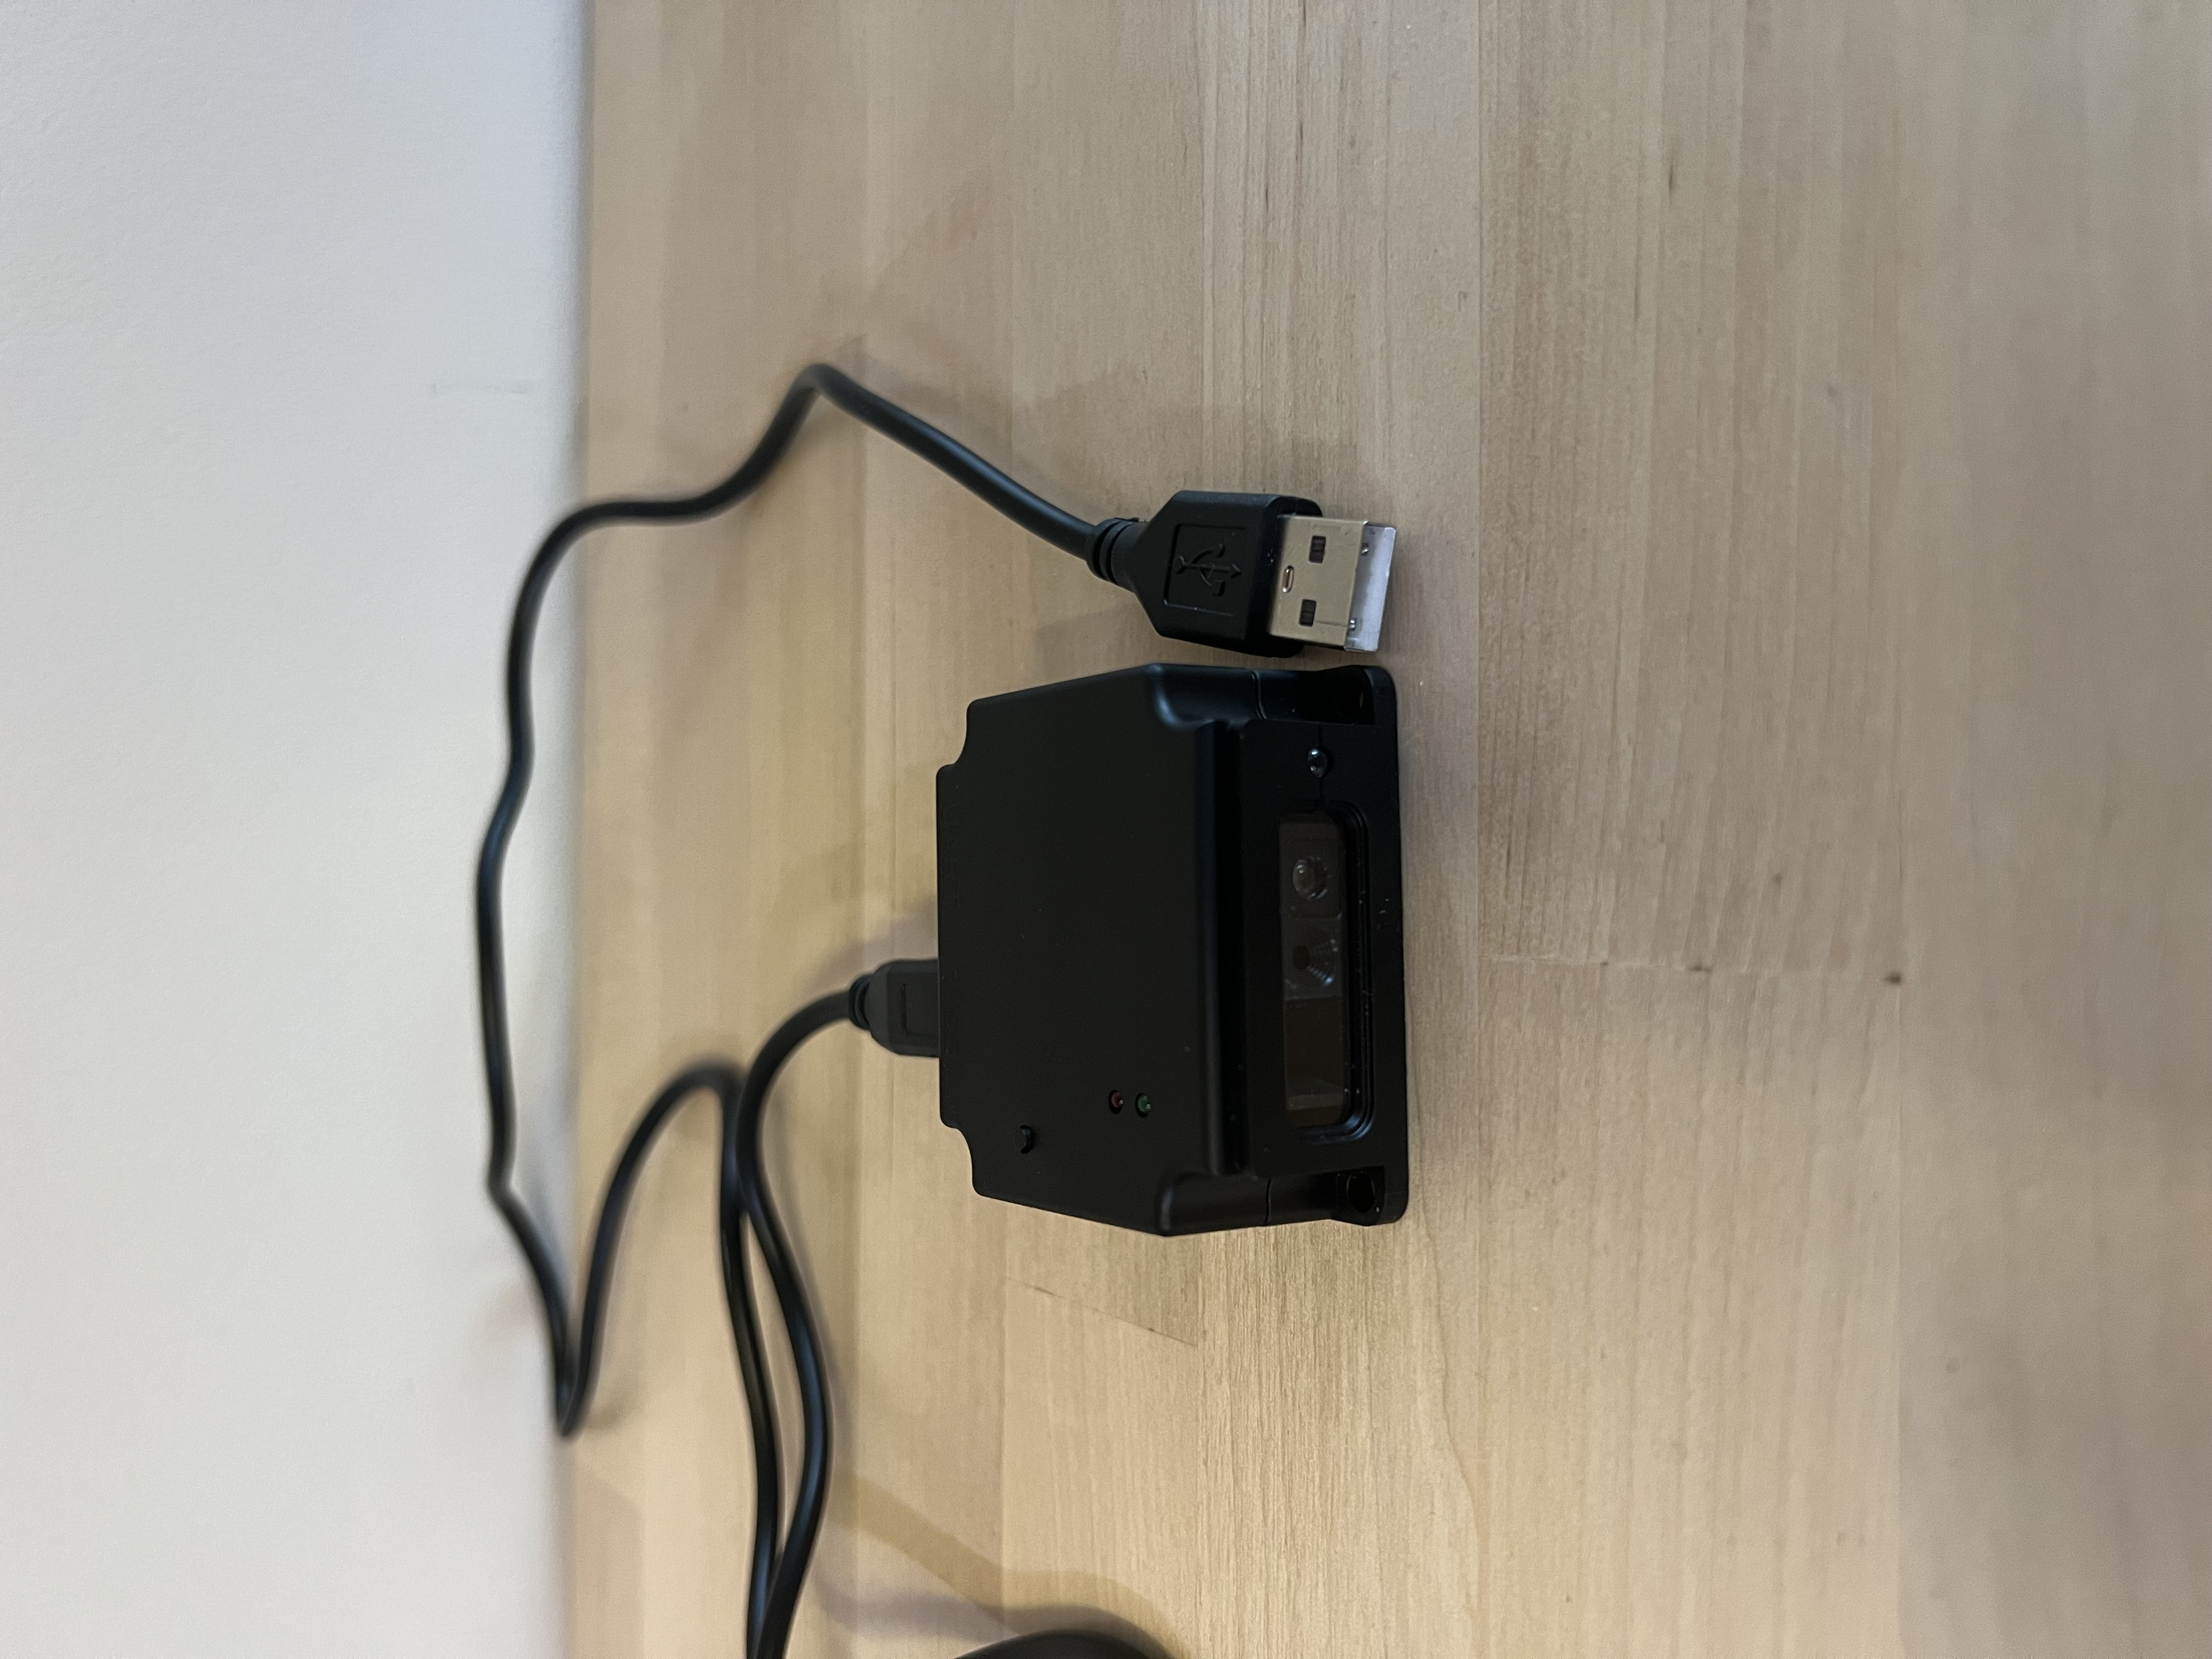
\includegraphics[width=\textwidth]{graphics/F24_scanner_back.jpeg}}
        \caption{Achterkant QR-scanner}
        \label{fig:scannerBack}
    \end{minipage}
    \hfill
    \begin{minipage}{0.32\textwidth}
        \centering
        \rotatebox{-90}{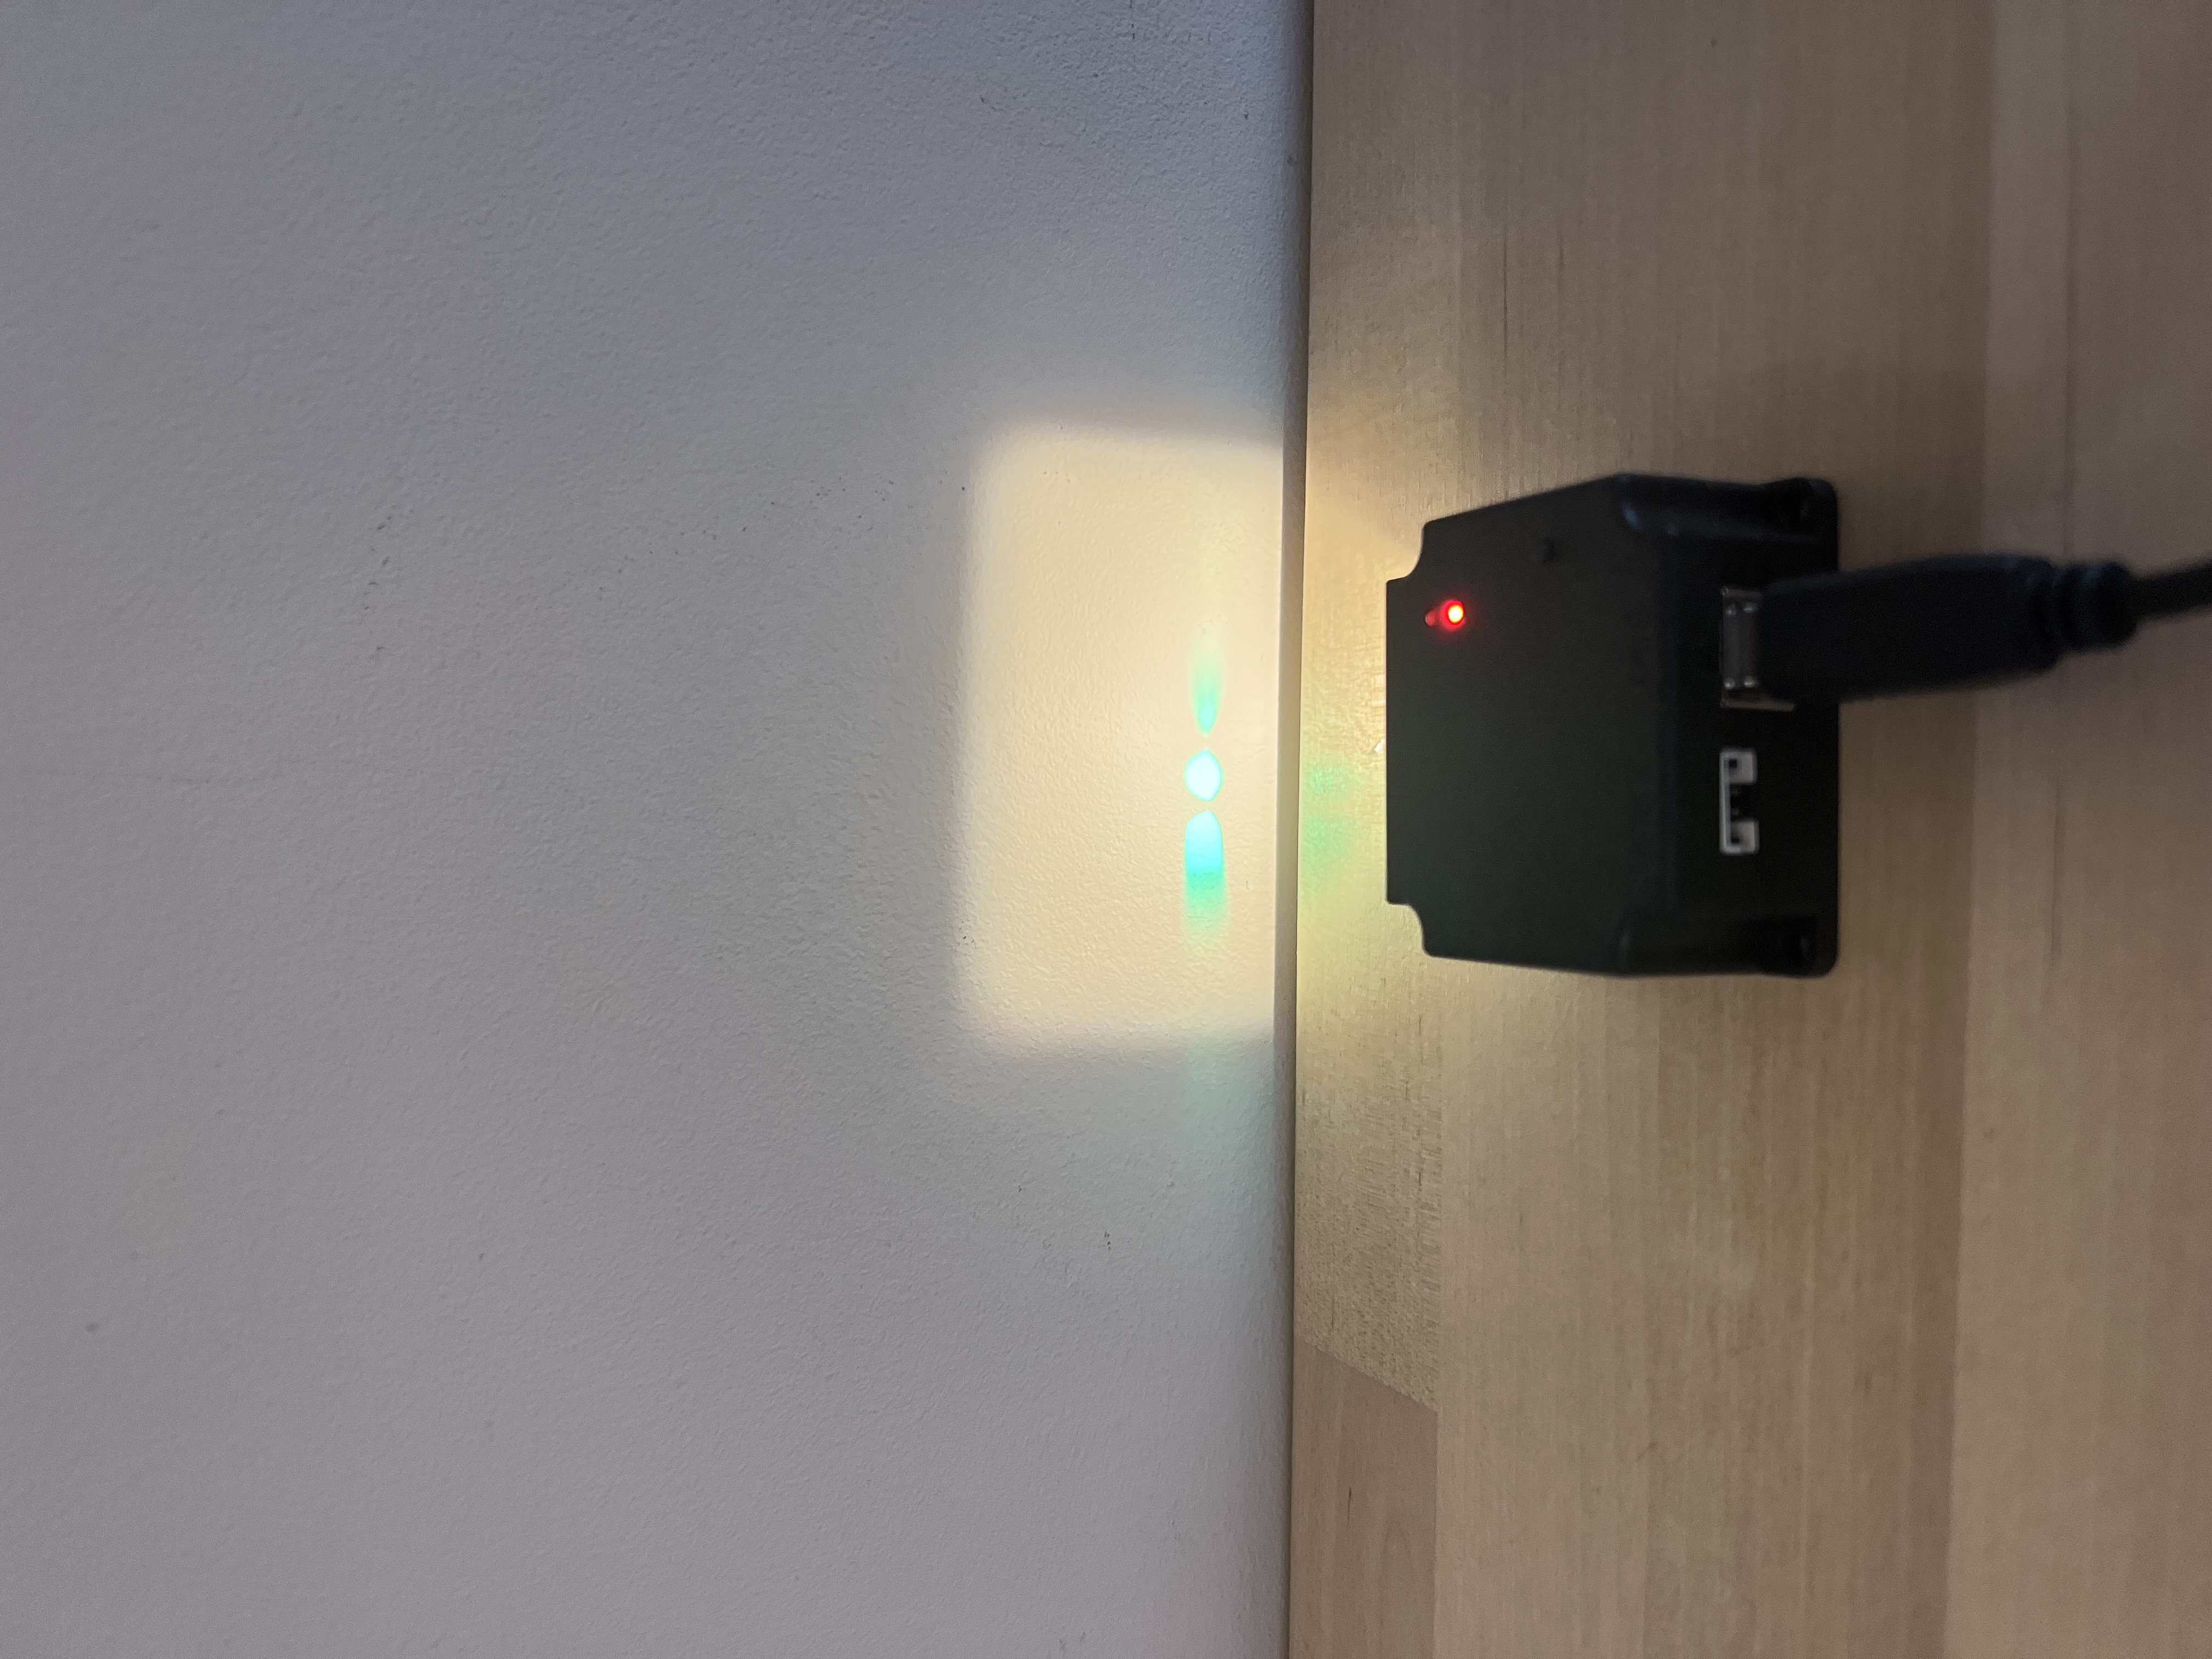
\includegraphics[width=\textwidth]{graphics/F25_scanner_front.jpeg}}
        \caption{Vooraanzicht QR-scanner}
        \label{fig:scannerFront}
    \end{minipage}
    \begin{minipage}{0.32\textwidth}
        \centering
        \rotatebox{-90}{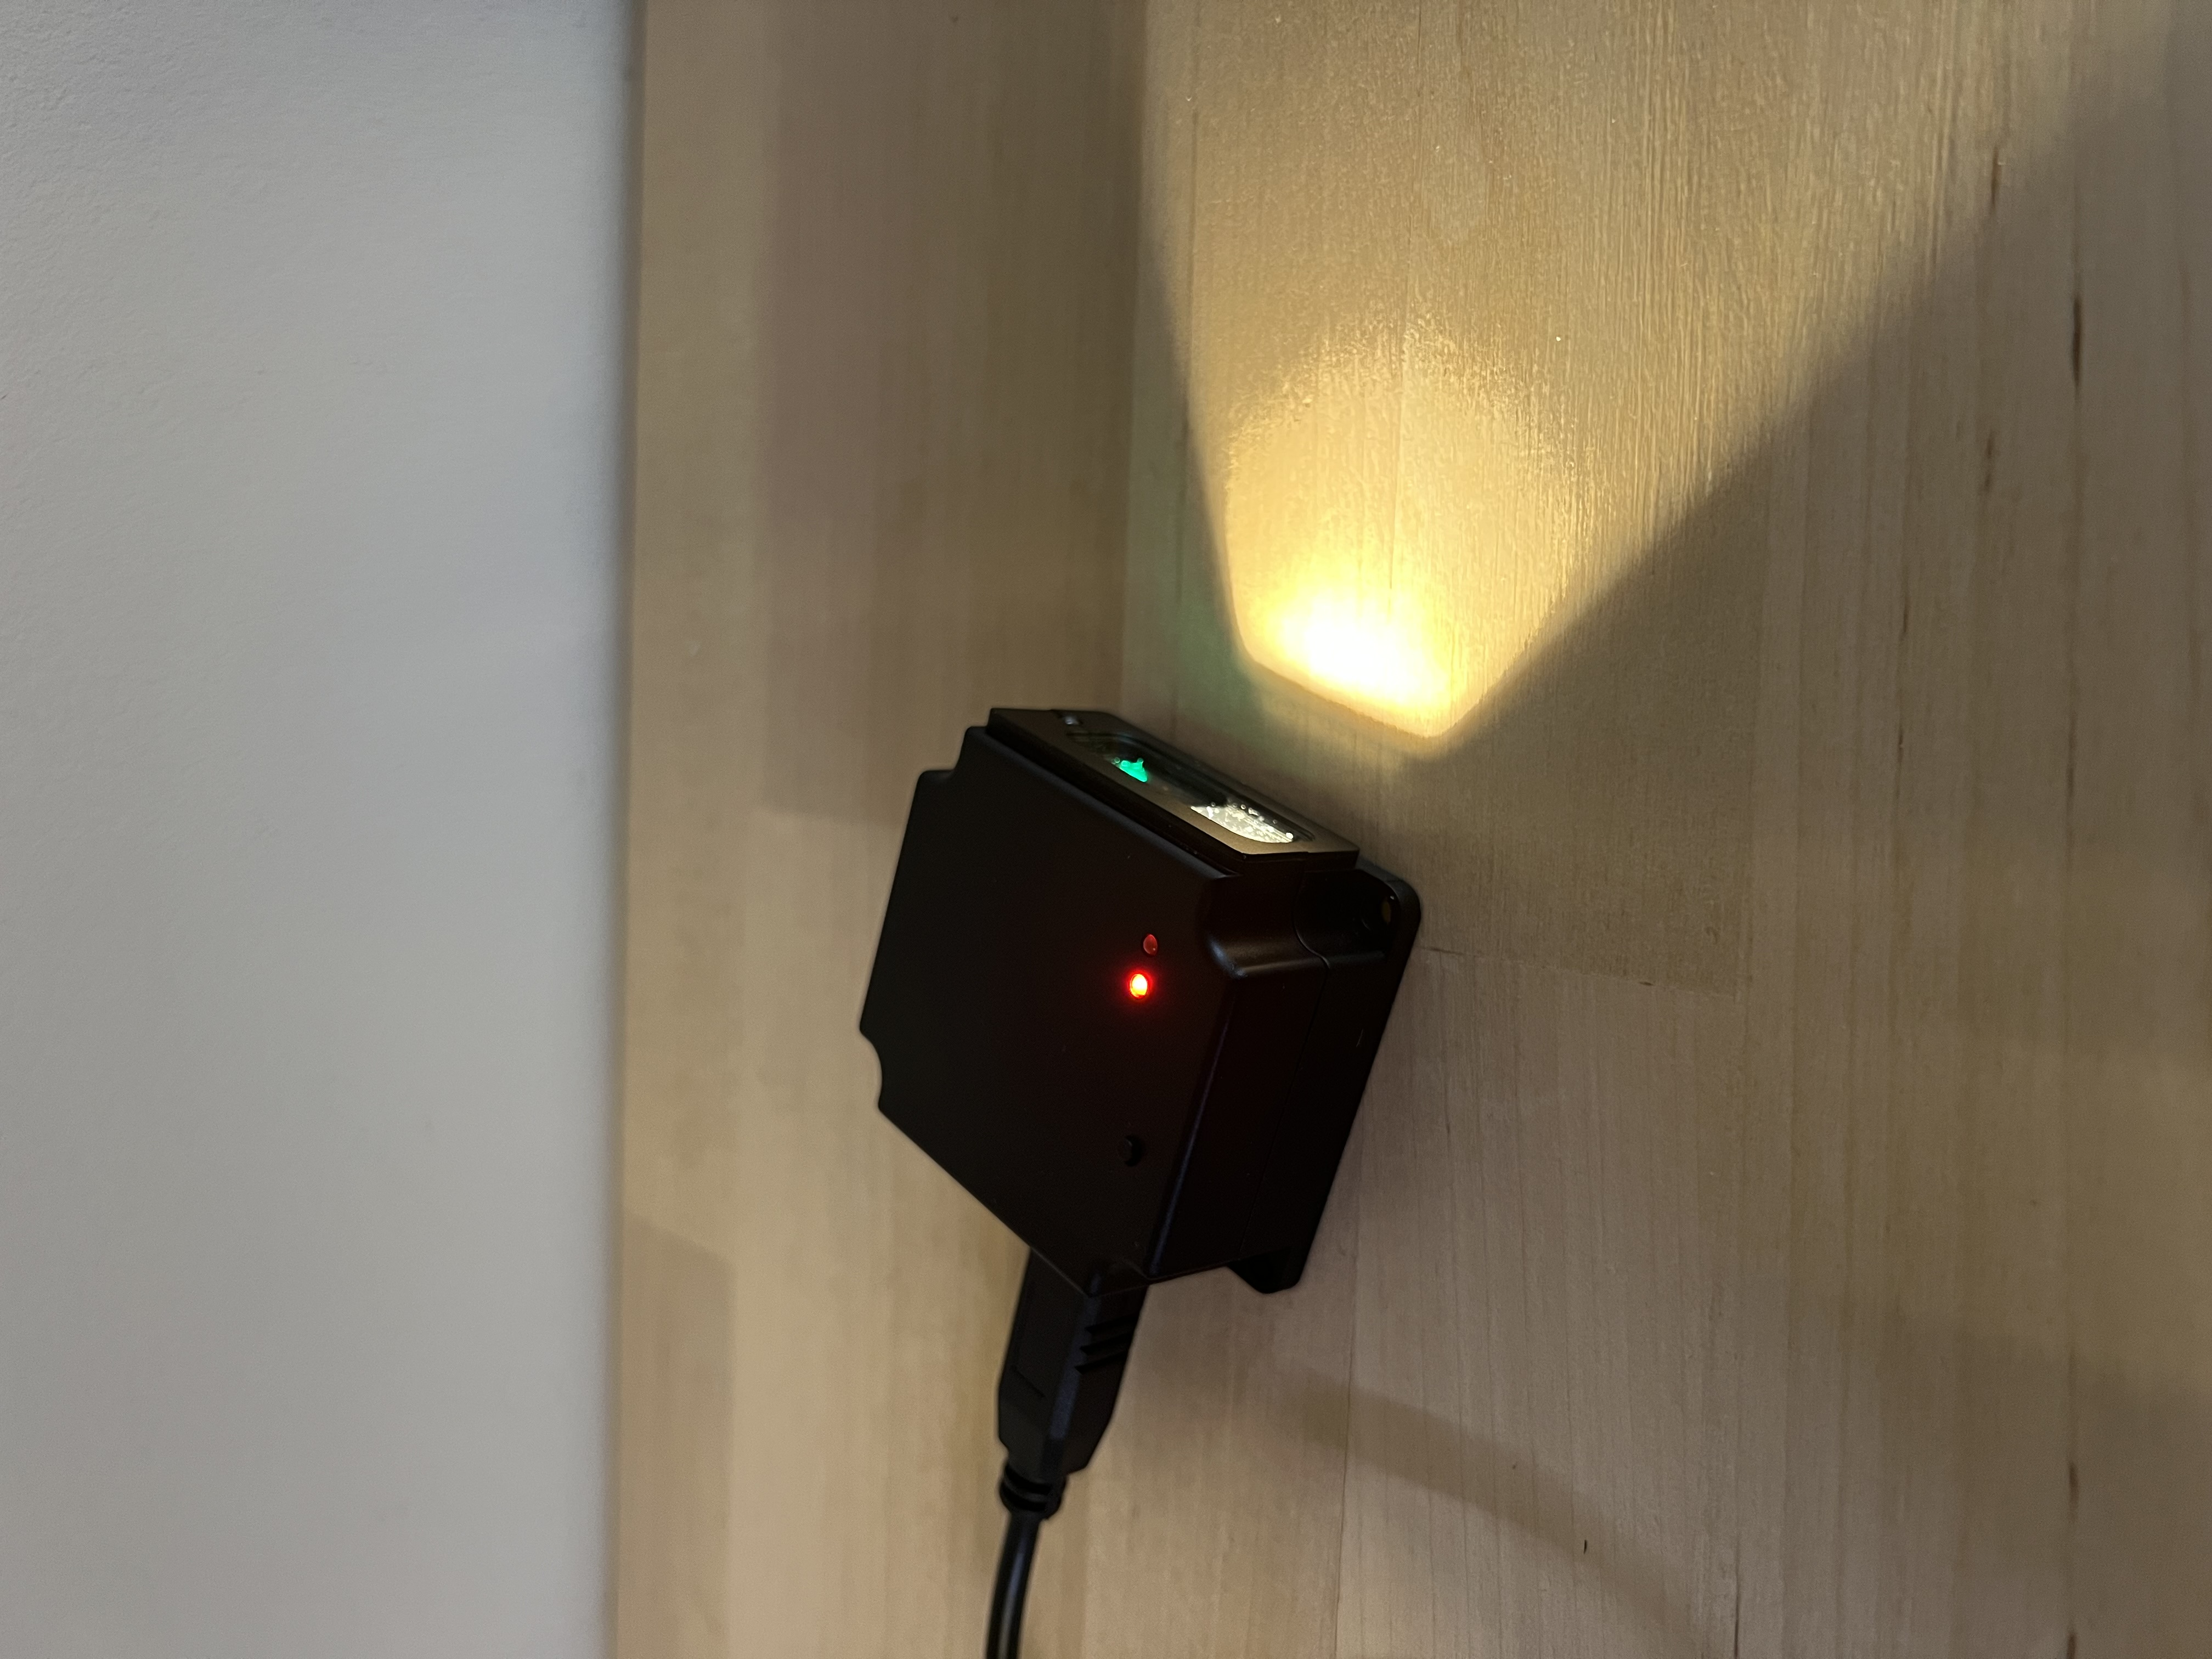
\includegraphics[width=\textwidth]{graphics/F26_scanner_side.jpeg}}
        \caption{Zijaanzicht QR-scanner}
        \label{fig:scannerSide}
    \end{minipage}
\end{figure}

\begin{figure}[h]
    \centering
    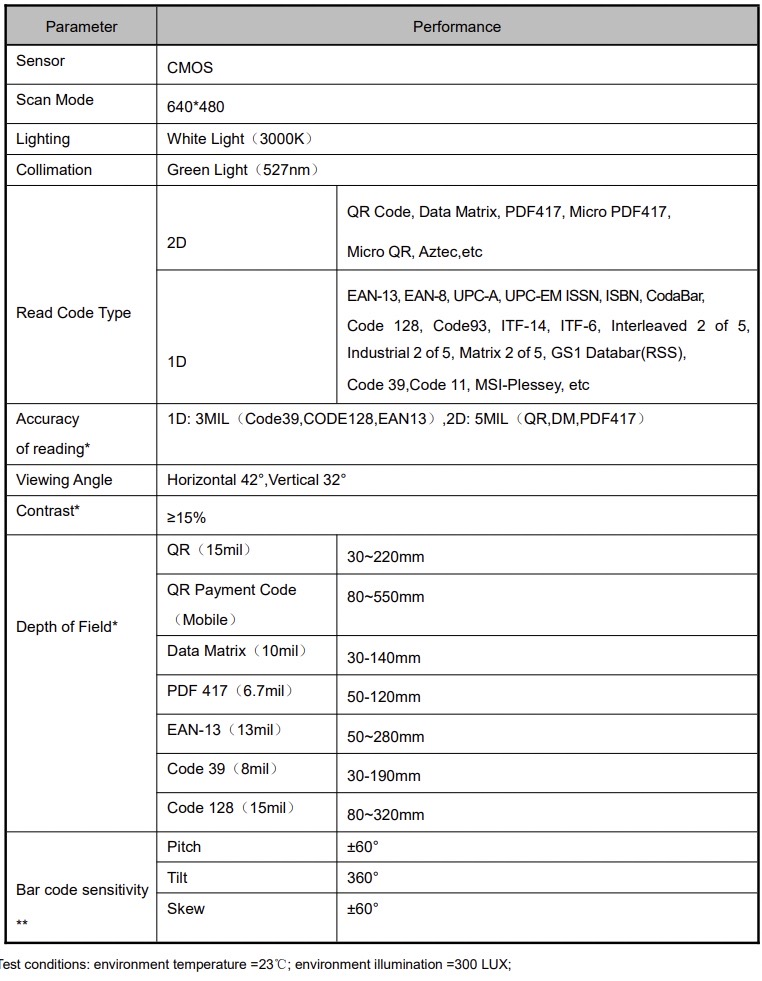
\includegraphics[width=0.8\textwidth]{graphics/F29_aangekochteQRScannerHandleiding.jpg}
    \captionsetup{justification=centering, singlelinecheck=false}    
    \caption{Handleiding aangekochte QR-code scanner.}
    \label{fig:handleidingNieuweQRScanner}
\end{figure}}

Om het experiment van de nieuwe QR-scanner zo goed mogelijk uit te voeren heb ik een nieuw script geschreven, dit script staat vermeld in listing \ref{lst:nieuweQR-codeData}. Deze gaat op dezelfde manier te werk als de huidige QR-code camera en gaat achteraf ook de opgehaalde data opslaan in een \ac{XLSX} bestand. Aan de hand van deze bestanden kunnen we de oude software en hardware vergelijken met de nieuwe om een duidelijke conclusie te maken in het hoofdstuk verwerking van resultaten.

\newpage

\begin{lstlisting}[language=Python, caption={Python script voor experiment van nieuwe QR-code scanner.}, label=lst:nieuweQR-codeData, numbers=left]
    import serial
    import time
    import pyzbar.pyzbar as pyzbar
    from datetime import datetime
    from datetime import timedelta
    from openpyxl import Workbook
    
    # De code opent de seriele poort van de scanner, in dit geval '/dev/tty.usbmodem2027300413411', op een baudrate van 9600
    port = '/dev/tty.usbmodem2027300413411'
    baud = 9600
    ser = serial.Serial(port, baud, timeout=1)
    
    # De variabele 'counter' houdt bij hoeveel QR-codes gescand zijn. De starttijd wordt vastgelegd met datetime.now().
    counter = 1
    start_time = datetime.now()
    
    # Een nieuw werkboek wordt aangemaakt met openpyxl.
    workbook = Workbook()
    worksheet = workbook.active
    
    # De eerste rijen van het werkblad krijgen labels voor de kolommen.
    worksheet['A1'] = 'Counter'
    worksheet['B1'] = 'Timestamp'
    worksheet['C1'] = 'Data'
    
    # Er wordt een while loop uitgevoerd die stopt nadat er 10 QR-codes zijn gescand.
    while counter <= 8:
        # De scanner leest de QR-code en de data wordt in de variabele 'data' opgeslagen.
        data = ser.readline().rstrip()
        if data:
            # De data wordt gedecodeerd met UTF-8 en opgeslagen in de variabele 'message'.
            message = data.decode('utf-8')
            # De huidige tijd wordt vastgelegd met datetime.now().
            timestamp = datetime.now()
            # De verstreken tijd sinds het begin van het scannen wordt berekend.
            elapsed_time = timestamp - start_time
            # Er wordt een datetime object aangemaakt met de huidige datum en de verstreken tijd.
            midnight = datetime.combine(datetime.today(), datetime.min.time())
            elapsed_datetime = midnight + elapsed_time
            # De tijd wordt in een leesbaar formaat opgeslagen in de variabele 'timestamp_str'.
            timestamp_str = elapsed_datetime.strftime('%H:%M:%S:%f')[:-3]
            # De data wordt geprint op het scherm.
            print(f'{counter} | {timestamp_str} | Data: {message}')
            # De data wordt toegevoegd aan het werkblad.
            worksheet.append([counter, timestamp_str, message])
            # De teller wordt verhoogd met 1.
            counter += 1
    
    # Het werkblad wordt opgeslagen als 'qr_codes_records_scanner.xlsx'.
    workbook.save('qr_codes_records_scanner_beschadigd_kaartje_120lux.xlsx')
    # De eindtijd van het scannen wordt vastgelegd met datetime.now() en geprint op het scherm.
    end_time = datetime.now()
    print(f"Counter reached {counter - 1}. Exiting program. Final time of scanning: {end_time - start_time}")
\end{lstlisting}

\subsection{Resultaten nieuwe QR-scanner experiment}
\label{sec:nieuweUitwerkingExperiment}

Hieronder bevinden zich de tabellen met daarin de eindresultaten van het experiment met de nieuwe QR-scanner. Er zijn telkens 50 QR-codes gescand met uitzondering van QR-codes in de beschadigde situatie.

\begin{table}[h]
    \centering
    \begin{tabular}{ c|c|c|c }
        \cline{2-4}
        & \textbf{\textit{QR-code op papier}} & \textbf{\textit{QR-code op gsm}} & \textbf{\textit{Verlichtingssterkte}} \\
        \cline{2-4}        
        \hline
        \textbf{\textit{1. Normaal}} & 157.496 s & 176.180 s & 120 lux \\
        \hline
        \textbf{\textit{2. Lichtinval}} & 177.737 s & 186.605 s & 100000 lux \\
        \hline
        \textbf{\textit{3. Donker}} & 158.847 s & 161.284 s & 5 lux \\
        \hline        
    \end{tabular}
    \captionsetup{justification=centering}
    \caption{De waarden in de tabel zijn uitgedrukt in seconden (s). Geef de resultaten weer van de nieuwe QR-scanner experiment.}
    \label{tab:3expeQR-scanner}
\end{table}

Het experiment dat beschadigde QR-codes omvat zal doorgaan met een set van acht QR-codes die beschadigd of onleesbaar gemaakt zijn. Deze QR-codes zijn zichtbaar op figuur \ref{fig:beschadigdeQR-codes} en zijn gerangschikt op basis van toenemende mate van beschadiging.

\begin{table}[h]
    \centering
    \begin{tabular}{ c|c }
        \cline{2-2}
        & \textbf{\textit{Beschadigd}} \
        \cline{2-2}
        \textbf{\textit{QR-code 1}} & 3,777 s \
        \cline{2-2}
        \textbf{\textit{QR-code 2}} & 11,953 s \
        \cline{2-2}
        \textbf{\textit{QR-code 3}} & 14,995 s \
        \cline{2-2}
        \textbf{\textit{QR-code 4}} & 14,995 s \
        \cline{2-2}
        \textbf{\textit{QR-code 5}} & 22,390 s \
        \cline{2-2}
        \textbf{\textit{QR-code 6}} & 25,340 s \
        \cline{2-2}
        \textbf{\textit{QR-code 7}} & 29,454 s \
        \cline{2-2}
        \textbf{\textit{QR-code 8}} & 32,495 s \
        \cline{2-2}
    \end{tabular}
    \captionsetup{justification=centering}
    \caption{De waarden in de tabel zijn uitgedrukt in seconden (s). De verlichtingssterkte bij deze uitwerking is 120 lux. De QR-codes in kwestie zijn te vinden in figuur \ref{fig:beschadigdeQR-codes}.}
    \label{tab:omgezette_tabel2}
\end{table}

\newpage

\section{Ontwikkeling van chatbot}%

De chatbot maken was een uitdaging binnen de requirements analyse en de tijdslimiet van deze bachelorproef. Echter wou ik deze wel uitwerken zodat er een QR-code op de eenvoudigste manier kan gerecupereerd worden. Om dit doel te bereiken waren twee eigenschappen enorm belangrijk. Een gebruiksvriendelijke interface hanteren alsook een makkelijke integratie in eender welk mediaplatform is noodzakelijk. Met deze twee cruciale kenmerken in het achterhoofd, ben ik naar chatbot platformen gaan zoeken. Veel bedrijven zoals Google of Microsoft bieden interessante dienstverleningen aan om een eigen chatbot te ontwikkelen, maar de prijsklasse van deze platformen liggen buiten het opgegeven budget.

Het zoeken van een chatbot service die aan de vooraf opgestelde eisen en voorwaarden voldoet, was niet eenvoudig. Voor deze Proof-Of-Concept heb ik de service genaamd ‘BotPress’ gekozen. BotPress maakt gebruik van Node.js en een modulaire architectuur. Dit maakt het ons eenvoudiger aangezien de business logica en de back-end van de Lockit Rentals applicatie ook gecodeerd is in dezelfde taal. Het biedt ook functies aan, zoals machine learning, natuurlijke taalverwerking, contextuele dialoogbeheer, integratie met externe services en analyse van gebruikersgedrag. Dit alles binnen een gratis opstartkost met maximaal 1000 conversaties per maand. Dankzij deze voordelen kunnen we de kennis verder zetten en de aangepaste modules integreren.

Het gebruik van BotPress is eenvoudig maar kan indien nodig voor genoeg diepgang zorgen. De conversatie of workflow bestaat uit verschillende blokken wat ‘Nodes’ wordt genoemd. Hierin kunnen vijf types van acties gebeuren zoals weergegeven in figuur \ref{fig:botpressActies}. Als eerste actie kan de eindgebruiker een voorgeprogrammeerd bericht ontvangen. Dit bericht kan uit verschillende types bestaan: tekst, video, audio, afbeeldingen of locatie zijn hier voorbeelden van. In een tweede actie binnen een Node blok kan er een interactie aangegaan worden met de eindgebruiker. Bij deze optie kan of mag de gebruiker een antwoord geven op een vooraf gedefinieerde vraag. Dit antwoord wordt nadien bewaard in een variabele die aangemaakt is binnen de workflow figuur \ref{fig:botpressVariables}. Het laten uitvoeren van eigen geschreven of \ac{AI} gegenereerde code is de derde actie die binnen de werkomgeving kan worden aangemaakt. Dit laat toe om opdrachten uit te sturen naar andere externe diensten buiten het platform. Bij de implementatie van de Lockit Rentals Chatbot maken wij hier uitgebreid gebruik van om te kunnen communiceren met de Lockit Rentals applicatie. De voorlaatste stap markeert de overgang tussen verschillende 'Nodes', waarbij er meerdere mogelijkheden zijn om verder te gaan met het gesprek. Hierdoor krijgt de eindgebruiker de vrijheid om verschillende routes te verkennen en het gesprek verder op maat te maken om zoveel mogelijk informatie te vergaren. De laatste actie die het minst gebruikt is binnen onze toepassing is een \ac{AI} task. 
Belangrijk om weten is dat er geen beperkingen zijn met betrekking tot de volgorde waarin de vijf acties uitgevoerd worden. Aan de hand van een gestructureerd stroomdiagram heb ik de chatbot opgebouwd weergegeven in figuur \ref{fig:workflowBotPress}. 

\subsection{Stappen om QR-code terug te winnen via chatbot}

Hieronder volgt een voorbeeld hoe je als festivalganger een QR-code kan terugwinnen via de chatbot. Deze stappen worden later gevisualiseerd in sectie \ref{sec:resultatenChatbot}
\newline

Primaire actor: Festivalganger die zijn of haar locker niet kan openen vanwege een verloren QR-code.
\newline
Secundaire actor: Chatbot dat is ontworpen om de festivalganger te helpen de verloren QR-code terug te geven.
\newline
Normaal verloop:

\begin{enumerate}
    \item De festivalganger typt een bericht om de chatbot te activeren.
    \item De festivalganger selecteert de optie "verloren QR-code".
    \item De chatbot haalt de huidige festivals op waar de lockers actief staan en presenteert deze aan de festivalganger via een keuze menu. \ref{ophalenActieveFestivals}
    \item De festivalganger selecteert het juiste festival waarbij hij/zij de locker heeft aangekocht.
    \item De chatbot vraagt naar het e-mailadres van de festivalganger om de QR-code op te sturen.
    \item De festivalganger verstrekt het juiste e-mailadres.
    \item De chatbot stuurt een verzoek naar de achterliggende service met het zonet ingegeven emailadres. \ref{versturenRequestEmail}
    \item Het systeem zal de QR-code ophalen en een mail versturen. \ref{ophalenQR}
    \item De chatbot krijgt het antwoord van het verzoek binnen en geef een gepaste melding.
ac
    \item De festivalganger ontvangt de QR-code en kan deze gebruiken om zijn of haar locker te openen.
\end{enumerate}

Alternatieve verlopen:
\newline
Hierbij zal de chatbot een gepaste foutmelding geven en de vraag opnieuw stellen. De chatbot zal er alles aan doen om de eindgebruiker genoeg informatie te verschaffen zodanig hij/zij zijn weg vindt in de conversatie.

\subsection{Ophalen evenementen waarop lockers actief zijn}
\label{ophalenActieveFestivals}
De chatbot zal de vraag stellen om een evenement aan te duiden in de chat. Een lijst van alle actieve evenementen waarop de lockers actief staan is hiervoor nodig. Deze actie wordt uitgevoerd in een stroomdiagram aan de hand van eigen geschreven code. Het antwoord op dit verzoek wordt bewaard in vooraf gedefinieerde lijsten. Deze code is voorgesteld in listing \ref{lst:botpressActie1}.

\begin{lstlisting}[language=Python, caption={Code blok geschreven in javascript om een actie van botpress uit te voeren.}, label=lst:botpressActie1, numbers=left]
    const response = await axios.get('https://europe-west2-lockit-testing.cloudfunctions.net/getActiveShops')
    
    const festivalsToAdd = response.data.map((festival) => festival.name)
    console.log(festivalsToAdd)
    // add the new festivals to the list
    workflow.ListOfFestivals = festivalsToAdd
    workflow.ListOfFestivalsObj = response.data
\end{lstlisting}

De ophaling van alle actieve evenementen verloopt in de backend van de Lockit Rentals applicatie. Dit wordt geconverteerd naar duidelijke objecten om zo weer te geven in de chat.
Methode \ref{lst:botpressActie2}, waarin men informatie verkrijgt van festivals waar lockers actief staan.
\begin{lstlisting}[language=JavaScript, caption={Methode waarin festivals worden ogpehaald waar lockers actie zijn.}, label=lst:botpressActie2, numbers=left]
    import * as functions from 'firebase-functions';
    import * as admin from 'firebase-admin';
    
    export const shopOverview = functions
    .region('europe-west2')
    .https.onRequest(async (req, resp) => {
        const db = admin.firestore();
        
        const activeShops = await db
        .collection('shop')
        .where('status', '==', 'LIVE')
        .get();
        
        resp
        .status(200)
        .send(activeShops.docs.map((doc) => ({ id: doc.id, ...doc.data() })));
    });
\end{lstlisting}

\subsection{Verzoek sturen naar backend om verloren QR-code op te halen}
\label{versturenRequestEmail}

Eénmaal de chatbot het e-mailadres goed heeft ontvangen kan het proces van het terugwinnen van een QR-code in werking treden. De chatbot voert een taak uit dat weergegeven wordt in listing \ref{lst:botpressActie3}. 

\begin{lstlisting}[language=JavaScript, caption={Een blok uitvoerbare code geschreven in javascript in een actie van Botpress. Deze code zal een verzoek uitsturen en het antwoord hiervan capteren.}, label=lst:botpressActie3, numbers=left]
    const response = await axios
    .post('https://europe-west2-lockit-testing.cloudfunctions.net/recoverLostCode', {
        shopId: workflow.FestivalNameObj['id'],
        email: workflow.Emailadress
    })
    .then((response) => {
        workflow.EmailSend = true
    })
    .catch((error) => {
        if (error.response && error.response.status === 404) {
            workflow.RecoveQr = "I couldn't find any email address associated with a purchased QR code. Please try again."
        } else if (error.response && error.response.status === 500) {
            workflow.RecoveQr = 'Something bad happend..... :^('
        } else {
            console.log(error)
        }
    })
\end{lstlisting}

\subsection{Ophalen van QR-code en aanmaken e-mail}
\label{ophalenQR}

Dit verzoek zal opnieuw afgehandeld worden in de backend van de Lockit Rentals applicatie. Het uitvoeren van onderstaande code \ref{lst:botpressActie4} zal de QR-code ophalen uit de reservatie tabel. Het antwoord waarin hij aangeeft dat de QR-code succesvol is opgehaald en de herstel email zullen verzonden worden. Op deze manier kan de chatbot een gepaste actie voorzien om de gebruiker erop te wijzen dat deze email onderweg is. 

\begin{lstlisting}[language=JavaScript, caption={Het ophalen van de bijhorende QR-code, indien dit gelukt is een opmaken en bewaren in de databank.}, label=lst:botpressActie4, numbers=left]
    const shopSnap = await db.collection('shop').doc(recoveryData.shopId).get();
    
    /**
    * If we can't find the shop, no point in searching for the reservation
    */
    if (!recoveryData.shopId || !shopSnap.data()) {
        resp.status(500).send();
    }
    
    if (recoveryData.email) {
        const reservationsSnap = await shopSnap.ref
        .collection('reservations')
        .withConverter(converter<ShopReservation>())
        .where('customerEmail', '==', recoveryData.email)
        .get();
        for (const reservationSnap of reservationsSnap.docs) {
            const reservation: ShopReservation = reservationSnap.data();
            await db
            .collection('mail')
            .doc()
            .create({
                to: reservation.customerEmail,
                message: {
                    subject: '🎉 Your locker for ' + reservation.shopName,
                    html: constructLiveSaleEmail(
                    reservation.lockerNumber + '',
                    reservation.optionName,
                    reservation.shopName,
                    reservation.customerName,
                    reservation.lockerType,
                    reservation.optionLocationName,
                    reservation.accessCode + ''
                    ),
                },
            });
        }
        if (reservationsSnap.size > 0) {
            resp.status(201).send();
        } else {
            resp.status(404).send('email adress not found');
        }
    } else if (recoveryData.phone) {
        console.log('tel reached');
    }
    
    resp.status(200).send();
});
\end{lstlisting}

\subsection{Versturen van aangemaakte herstel email}
\label{versturenQRcode}

Om de aangemaakte email met daarin de gerecupereerde QR-code te verzenden naar de eindgebruiker is echter een ander verhaal. De aangemaakte email wordt bewaard in een tabel ‘customerEmail’. Om deze mail automatisch te detecteren gebruiken we de extentie binnenin Firebase genaamd ‘Tigger email’. Deze extentie zorgt voor het detecteren van emails die aangemaakt zijn binnen de tabel ‘customerEmail’. De extentie kan zo nog een derde provider aanspreken genaamd ‘Mail Sender’ die ervoor zal zorgen dat de email naar de desbetreffende correspondent verstuurd wordt. Via deze tool kunnen we alles analayseren wat er precies  gebeurt met de verstuurde email. 

\begin{figure}[h]
    \centering
    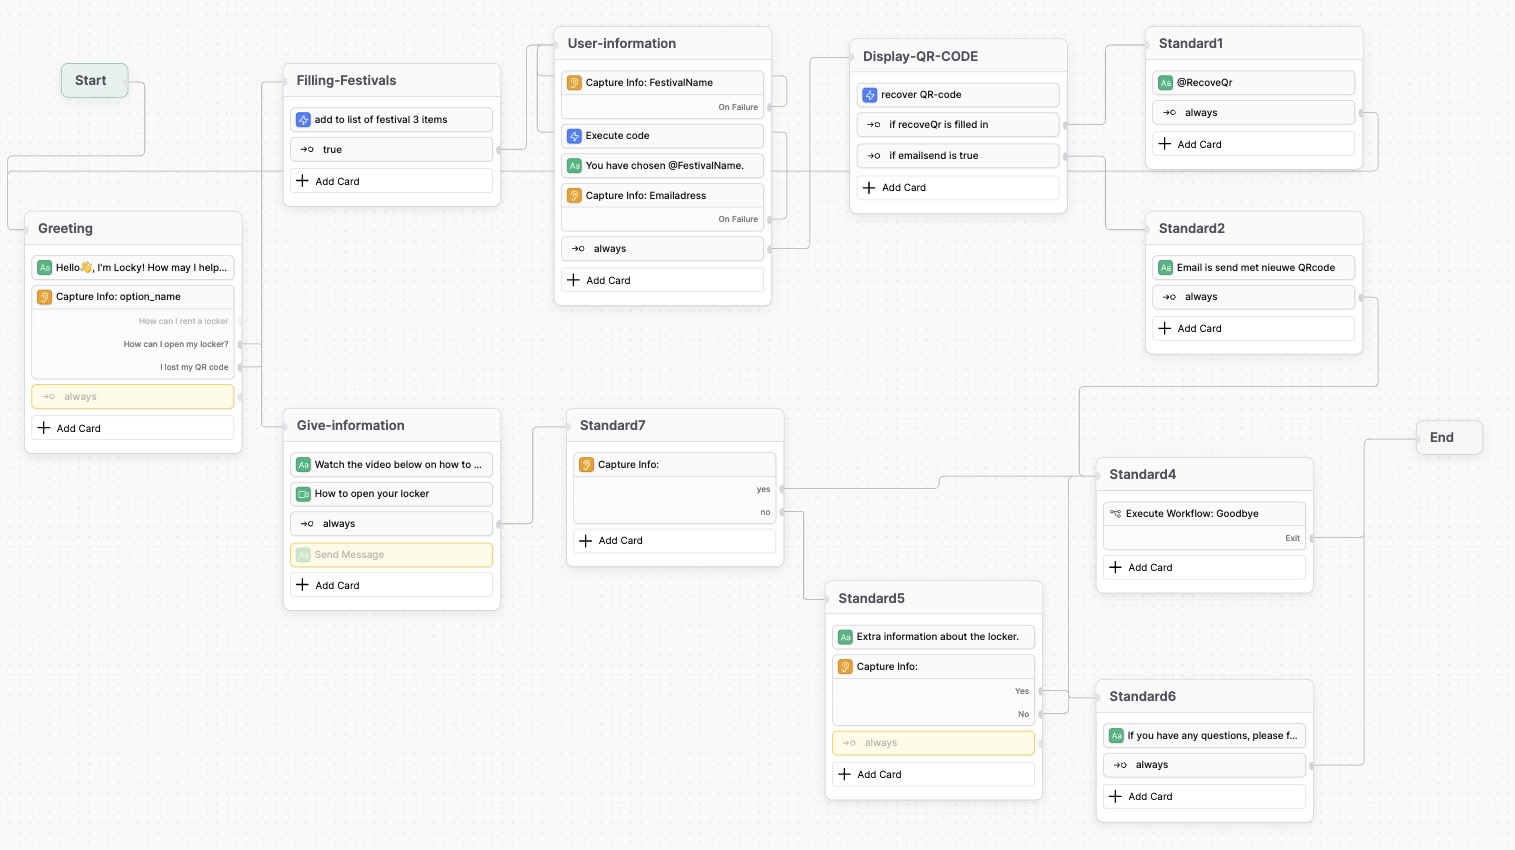
\includegraphics[angle=90, width=0.9\textwidth]{graphics/F36_workflowBotPress.jpg}
    \captionsetup{justification=centering}    
    \caption{De workflow van de Lockit Rentals Bot gemaakt in BotPress.}
    \label{fig:workflowBotPress}
\end{figure}

%todo: figuur aanvullen van volledig model botpress
\begin{figure}[h]
    \centering
    \begin{minipage}{0.45\textwidth}
        \centering
        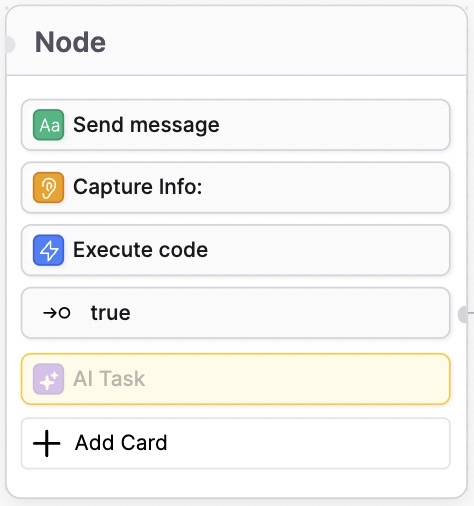
\includegraphics[width=\textwidth]{graphics/F31_botpress_Acties.jpg}
        \caption{Representatie BotPress Node en vijf verschillende acties.}
        \label{fig:botpressActies}
    \end{minipage}
    \hfill
    \begin{minipage}{0.45\textwidth}
        \centering
        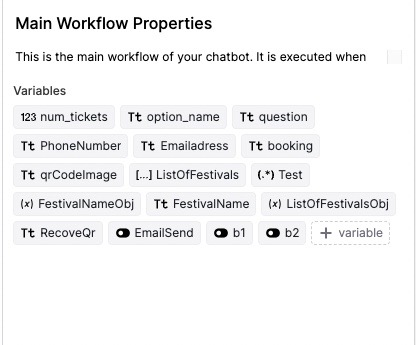
\includegraphics[width=\textwidth]{graphics/F32_botpress_Variables.jpg}
        \caption{Alle variabelen die binnen de workflow zitten voor de Lockit Rentals chatbot.}
        \label{fig:botpressVariables}
    \end{minipage}
\end{figure}














